%ここから
% \documentclass[12pt,a4j]{jarticle}
\documentclass[12pt,a4j,uplatex]{jarticle} % 縦書き用
\usepackage[dvipdfmx]{graphicx}
\usepackage{float}
\usepackage{times}
\usepackage{amsmath}
\usepackage{url}
\usepackage[titletoc,title]{appendix}
\usepackage{plext} % 縦書き用
\usepackage[a4paper]{geometry} % 縦書き用

\pagestyle{plain}
\setlength{\textwidth}{150mm}
\setlength{\textheight}{230mm}
\setlength{\oddsidemargin}{+4.6mm}
\setlength{\topmargin}{-10mm}
\setlength{\footskip}{20mm}
\newfont{\ssf}{cmssbx10 scaled\magstep3}

\nonstopmode
%日本語用に jplain 英語の場合は plain にすること
% \bibliographystyle{jplain}
\bibliographystyle{esdhcu}

%何か追加したい場合,ここから追加すること
\usepackage{newenum}
\usepackage{listings}
%\usepackage[dvips]{graphicx}
\usepackage[dvipdfmx]{graphicx,xcolor}
\usepackage[T1]{fontenc}
\usepackage{lmodern}
%\usepackage{textcomp}
\usepackage{latexsym}
%\usepackage[fleqn]{amsmath}
%\usepackage{amssymb}
\usepackage{comment}
\usepackage{fancyvrb}
\usepackage{multicol}
\usepackage{newtxtext}
\usepackage{enumerate}
\usepackage{wrapfig}

%\setlength{\topskip}{0cm} % 段落間
%\setlength{\partopsep}{0cm} % 項目間

\makeatletter
\renewenvironment{itemize}
  {\ifnum \@itemdepth >\thr@@\@toodeep\else
   \advance\@itemdepth\@ne
   \edef\@itemitem{labelitem\romannumeral\the\@itemdepth}%
   \expandafter \list \csname \@itemitem\endcsname{%
      \iftdir
         \ifnum \@listdepth=\@ne \topsep.5\normalbaselineskip
           \else\topsep\z@\fi
         \parskip\z@ \itemsep\z@ \parsep\z@
         \labelwidth1zw \labelsep.3zw
         \ifnum \@itemdepth =\@ne \leftmargin1zw\relax
           \else\leftmargin\leftskip\fi
         \advance\leftmargin 1zw
      \fi
         \def\makelabel##1{\hss\llap{##1}}}%
   \fi}{\endlist}

\renewenvironment{description}
  {\list{}{\labelwidth\z@ \itemindent-\leftmargin
    \iftdir
    \leftmargin\leftskip \advance\leftmargin3\Cwd
    \rightmargin\rightskip
    \labelsep=0zw \itemsep\z@
    \listparindent\z@ \topskip\z@ \parskip\z@ \partopsep\z@
    \fi
    \let\makelabel\descriptionlabel}
    % \setlength{\parsep}{0mm} % 各段落間のスペース
    % \setlength{\parskip}{0mm} % 段落の前に入る縦方向スペース
    % \setlength{\itemsep}{0mm} % 項目間に入る縦方向スペース
  }{\endlist}
\renewcommand{\descriptionlabel}[1]{%
  \hspace\labelsep\normalfont\bfseries #1}
\makeatother

% \setlength{\itemindent}{0em}
% \setlength{\leftskip}{0em}
% \setlength{\listparindent}{-1em}

\newenvironment{dl}{
  % \setlength{\leftmargin}{0em}
  % \setlength{\leftskip}{0em}
  \begin{description}
    \setlength{\itemindent}{-1em}
    \setlength{\leftskip}{0em}
    % \addtolength{\itemindent}{1em}
    % \addtolength{\leftskip}{1em}
    \setlength{\parskip}{0mm} % 段落の前に入る縦方向スペース
    \setlength{\itemsep}{1mm} % 項目間に入る縦方向スペース
}{\end{description}}

\newenvironment{ol}{
  \begin{enumerate}
    \setlength{\itemindent}{0em}
    \setlength{\leftskip}{1em}
    % \addtolength{\itemindent}{-1em}
    % \addtolength{\leftmargin}{1em}
    % \setlength{\parsep}{0mm} % 各段落間のスペース
    \setlength{\parskip}{0mm} % 段落の前に入る縦方向スペース
    \setlength{\itemsep}{0mm} % 項目間に入る縦方向スペース
}{\end{enumerate}}

\newenvironment{ul}{
  \begin{itemize}
    \setlength{\itemindent}{0em}
    \setlength{\leftskip}{0em}
    % \addtolength{\leftmargin}{1em}
}{\end{itemize}}

\emergencystretch=1em

\renewcommand{\lstlistingname}{リスト}
\lstset{language=,%
        basicstyle=\ttfamily\footnotesize,%
        commentstyle=\textit,%
        classoffset=1,%
        keywordstyle=\bfseries,%
	% frame=single,
	frame=tRBl,
        framesep=5pt,%
	showstringspaces=false,%
        numbers=left,
        stepnumber=1,
        numberstyle=\footnotesize%
	}%

% 図と図の間のスペース
\setlength\floatsep{2truemm}
% 本文と図の間のスペース
\setlength\textfloatsep{2truemm}
% 本文中の図のスペース
\setlength\intextsep{0pt}
% 図とキャプションの間のスペース
\setlength\abovecaptionskip{1truemm}

% ぶら下げ
\newenvironment{hang}[1][\parindent]
  {\def\item{\par\hangindent=#1\noindent}}
  {\par}

% カンマの後,改行を許す
% \def\,{,\allowbreak}
% これを定義すると \cite に余計なカンマが入る.

% 縦棒の後,改行を許す
\def\|{\tt |\allowbreak}
% circumflex accent, caret, up arrow, hat, chevron
\def\hat{\mbox{\^{ }}}
% 鍵括弧
\def\sb#1{[#1]}
% 二重鍵括弧
\def\db#1{[\![#1]\!]}
% 三重鍵括弧
\def\tb#1{[\![\![#1]\!]\!]}
% 角括弧
\def\sa#1{\langle#1\rangle}
% 二重角括弧
\def\da#1{\langle\!\langle#1\rangle\!\rangle}
% 矢印
\def\->{\allowbreak\mbox{$\rightarrow$}\allowbreak}
% ・・・
\def\c...{\mbox{$\cdots\mbox{}$}}
% :=
\newcommand{\defeq}{\mathrel{\mathop:}=}

\newcommand{\NT}[1]{\ensuremath{\langle\mbox{#1}\rangle}\allowbreak}
\newcommand{\C}[1]{\mbox{\tt#1}}

% Hatの意味関数
\newcommand{\sH}[1]{\ensuremath{\mathcal{H}}\dlrBrack{\mbox{\tt#1}}}
\newcommand{\dlrBrack}[1]{\ensuremath{[\![#1]\allowbreak\!]}}

% Schemeの意味関数
\newcommand{\sS}[1]{\ensuremath{\mathcal{E}}\dlrBrack{\mbox{\tt#1}}}

% 式に含まれる自由変数の集合
\newcommand{\FV}[1]{\ensuremath{\mathcal{F}}\dlrBrack{\C{#1}}}

% ドットの前後に空白
\newcommand{\D}{\mbox{\tt\ .\ }}

% 継続付き関数
\newcommand{\FC}[2]{\mbox{\tt F.C #1\D#2}}

%追加ここまで

%ここまで

\renewcommand{\appendixname}{付録}
\usepackage{multirow}
\usepackage{here}
\usepackage{url}
\newcommand{\bhline}[1]{\noalign{\hrule height #1}}  
\newcommand{\bvline}[1]{\vrule width #1}  

\begin{document}
%行間の変更、必要ならば変えること
\setlength{\baselineskip}{8mm}
%タイトル製作用
%特に問題がないと思われるが、問題があれば 表紙.tex を編集すること
%ここから表紙開始
%%%%%%%%%%%%%%%%%%%%%%%%%%%%%%%%%%%%%%%%%%%%%%%%%%%%%%
%名前等,適度に変更すること
\renewcommand{\thepage}{}

\def\thethesis{令和\rensuji{5}年度 卒業論文}
\def\thetitle{深層学習を用いた\\セマンティックセグメンテーションによる\\水面領域抽出の精度評価}
\def\theauthor{中島 慶}

\def\thecover{
  \begin{center}
    {\huge
      \vspace*{4cm}
      \LARGE{\thethesis\\ }
    }\vspace{8mm}
    {\huge
      \LARGE{\thetitle}\\\vspace{2mm}
    }
  \end{center}
  \vspace{4cm}
  \begin{center}
    {\Large
      \noindent 広島市立大学 情報科学部 システム工学科 \\
      \vspace{3em}
      \noindent \hspace{4em}氏名\hspace{3em} \theauthor  \\
      \hspace{4em}指導教員\hspace{3em}島 和之 准教授\\
      \vspace{2em}
      2024年1月31日 提出\\
  }\end{center}
}

% ファイルの表紙と背見出し
\newgeometry{left=0cm,right=9mm,top=0cm}
\marginpar{\parbox<t>{11.5in}{\def\\{}\large\thethesis\hfill\thetitle\hfill\theauthor}}
\vspace{1in}
\thecover
\restoregeometry
\clearpage

% ファイル内表紙
\thecover
\clearpage
%%%%%%%%%%%%%%%%%%%%%%%%%%%%%%%%%%%%%%%%%%%%%%%%%%%%%%
%表紙ここまで

%目次製作用
%目次のスタイルを変えたい場合は、目次.texを編集すること
% \section{title} などで章等を追加した場合、勝手に目次も変更される
%ここから目次開始
%%%%%%%%%%%%%%%%%%%%%%%%%%%%%%%%%%%%%%%%%%%%%%%%%%%%%%
%このページは変更しないこと

\tableofcontents
\newpage
\setcounter{page}{1}
\renewcommand{\thepage}{\arabic{page}}

%%%%%%%%%%%%%%%%%%%%%%%%%%%%%%%%%%%%%%%%%%%%%%%%%%%%%%
%ここまで

%
%
%ここから本文書き始め
%本文.texで論文を書く
%本文.texで書く場合、 \begin{document} と \end{document} は不要
%なお、ここに直接本文を書いても良い
\section{序章}
\subsection{研究背景}
\label{1.1}
平成30年7月豪雨によって広島市で起こった土砂崩れや浸水による被害をはじめ、土砂災害は日本全国各地で年間平均1099件(昭和57年から令和4年まで)が発生している\cite{mlit}.
土砂災害の発生前には「降雨が続くにもかかわらず川の水位が低下する」や「崖から小石がパラパラと落ちる」といった前兆現象が起こることが確認されている\cite{zentyou}.
土砂災害の前兆現象を早期に検知し,住民に避難を促すことで人的被害の削減につながると期待されている.

そこで、前兆現象の一つである「降雨が続くにもかかわらず川の水位が低下する」に着目し,河川の監視カメラ画像から水位を推定する方法が提案されている\cite{watanabe}.
河川の水位は水位計を用いて計測する方法が一般的ではあるが、水位計にはコストの高さや整備の難しさといった問題がある。
このため,安価で整備が容易な監視カメラを用いた水位推定が水位計の代替案となっている\cite{seman}.

先行研究\cite{watanabe}では,河川の監視カメラ画像から多数の切抜画像を抽出し,畳込みニューラルネットワークで水面を判別し,
水位を推定する方法を提案した.しかし,訓練データと異なる日のテストデータに対しては,推定精度が低いという問題があった.

\subsection{研究目的}
\label{1.2}
本研究では,深層学習を用いたセマンティックセグメンテーションによって,
河川の監視カメラ画像から水面領域を抽出する手法(以下,SS 手法)を検討するため,
その精度を評価した.
深層学習を用いたセマンティックセグメンテーションでは,
一般的に,訓練データとしてアノテー ション付きの画像(以下,アノテーション画像)
が多数必要であり,かつ,精度に影響する.
ただし,多数のアノテーション画像を手作業で作成するには過大な労力がかかるので,
可能な労力で必要な精度を達成するため,半自動的な作成方法を検討する.

\clearpage
%%%%%%%%%%%%%%%%%%%%%%%%%%%%%%%%%%%%%%%%%%%%%%
\section{関連研究}
%Nurの研究について
\subsection{先行研究\cite{seman}}
\label{2.1}
Nurら\cite{seman}は,河川の監視カメラ画像から水面領域を抽出するために
畳込みニューラルネットワークに基づくセマンティックセグメンテーションを提案した.
DeepLabv3+\cite{deeplabv3+}とSegNet\cite{segnet}という二つのセマンティックセグメンテーション
向け畳込みニューラルネットワークで作成したモデルの領域抽出精度の比較を行った.
結果はDeepLabv3+を用いて作成したモデルの方が領域抽出精度が高いことが確認された.
また,高い抽出精度を示したDeepLabv3+モデルを用いて,河川の監視カメラ画像から
水位の推定と水位変動の観測を行った.推定した水位変動とセンサーで計測した水位
変動は強い相関関係を示し,セマンティックセグメンテーションは監視カメラ画像から水面領域を
抽出し,水位を推定する手段として有効であると報告した.

\clearpage
\subsection{DeepLabv3+}
\label{2.2}
DeepLabv3+\cite{deeplabv3+}はGoogle Research Teamによって考案されたセマンティックセグメンテーション
向け畳込みニューラルネットワークであり,旧バージョンのモデルから多くの改良が施された最先端のモデルの一つである.
DeepLabv3+は図\ref{figure:DeepLabv3+}に示すようにエンコーダ・デコーダ構造を持ち,
Atrous convolutionを備えている.

Atrous convolutionは一般的な畳込み層より大きい受容野を持ち,効率的に畳込みすることが可能な層である.
また,それは式(1)のように表される.
式(1)の,$y[i]$は出力,$w[k]$は長さkのフィルタ,$x$は入力である特徴マップ,$r$はAtrous rate
を表す.

\begin{equation}
  \label{filter}
  \begin{center}
    $y[{i}]=\displaystyle\sum_{k}x[{i+r\cdot k}] \cdot w[{k}]$
  \end{center}
\end{equation}

\begin{figure}[ht] 
  \begin{center}
    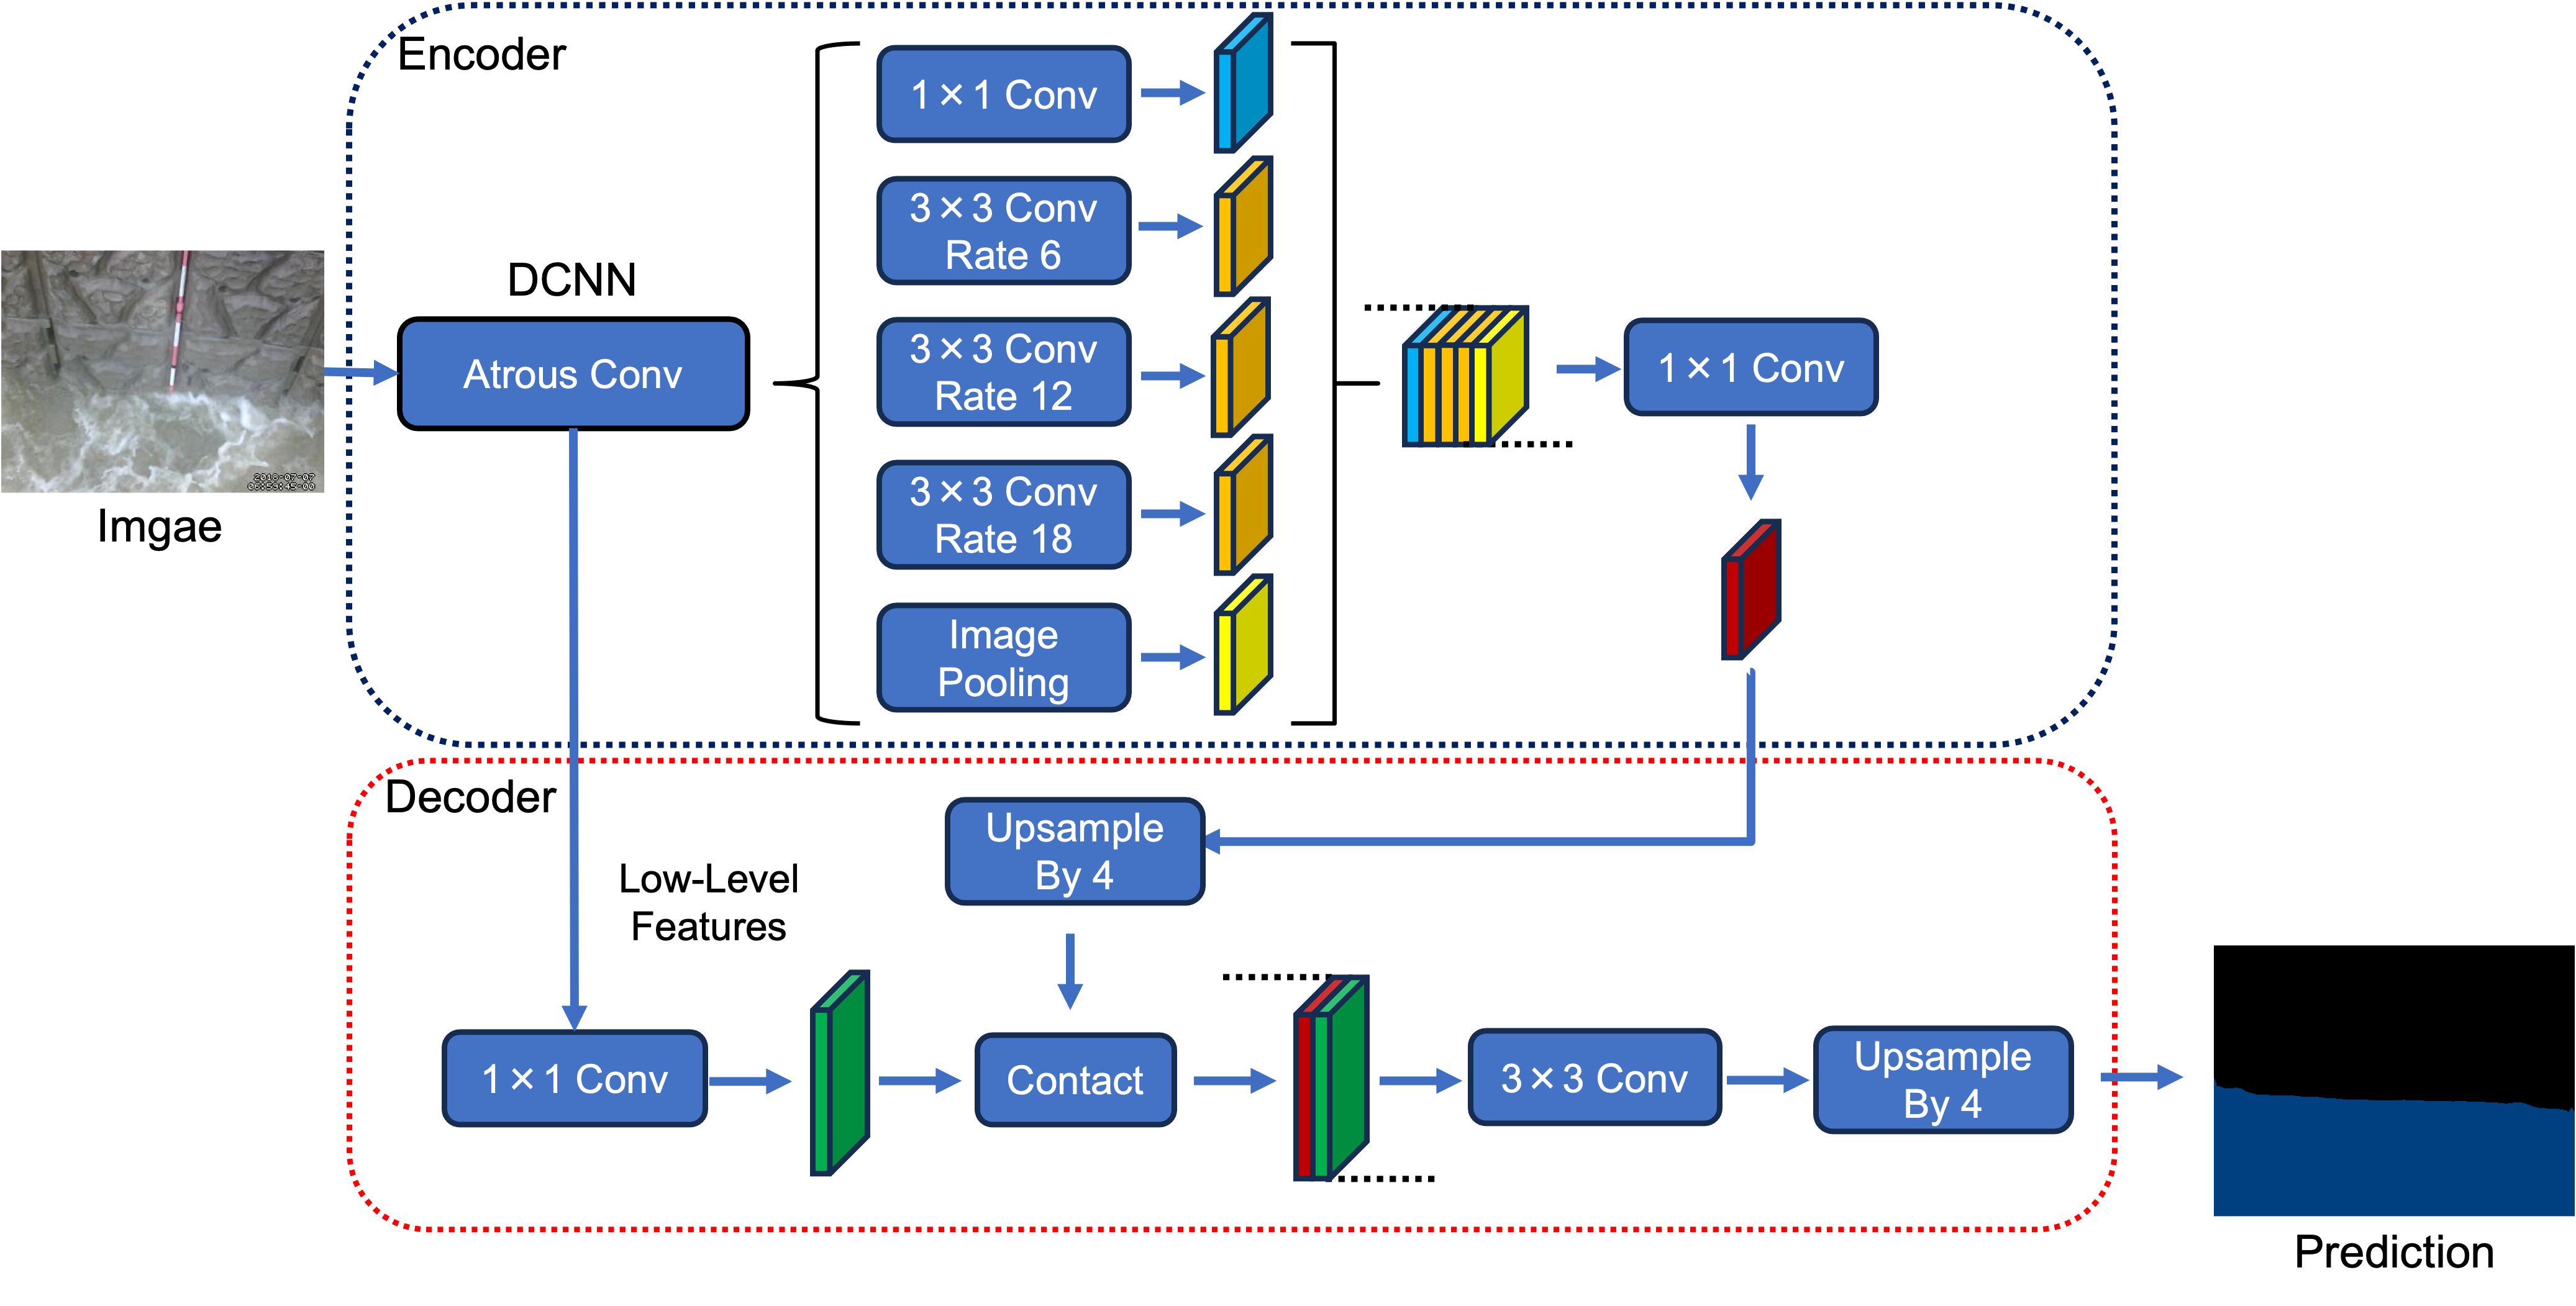
\includegraphics[width=\linewidth]{image/DeepLabv3+.png}
  \end{center}
  \caption{DeepLabv3+モデル}
  \label{figure:DeepLabv3+}
\end{figure}
\clearpage
%%%%%%%%%%%%%%%%%%%%%%%%%%%%%%%%%%%%%%%%%%%%%%
\section{先行研究\cite{watanabe}}
\subsection{概要}
\label{3.1}
先行研究\cite{watanabe}は,土砂災害の前兆現象の一つである「降雨が続くにもかかわらず
川の水位が低下する」現象に着目した.河川の監視カメラ画像を図\ref{kirinuki}の
ように切り抜き,切抜画像が水面かどうかを畳込みニューラルネットワークによって
判別を行い,判別されるときに出力される水面クラスのソフトマックス値と元画像の縦座標値を用いて
水位の変動を推定した.深層学習を用いて推定した水位変動と実際の水位変動
との相関を評価をした.

\subsection{画像の切り抜きとラベル付け}
\label{3.2}
河川の監視カメラ画像の幅を5等分(幅64高さ×240pixel)になるよう
に切り分け,そのうち,水位計測ポールを含む
中央の列を除外を行った.残った各4列に対して,
高さを元の河川画像を5等分した大きさ(各48pixel)となるように,幅64×
高さ48pixelの画像を縦に8pixelずつ移動させて,最下段まで切り抜きを行った.
切り抜いた画像に対して,以下に示す3つのクラスに分類してラベル付けを行った.
\begin{description}
    \item・ 「水面」  : 水面が写っている画像
    \vspace{-2mm}
    \item・ 「壁面」  : 壁面が写っている画像
    \vspace{-2mm}
    \item・ 「その他」 : 水面と壁面の両方が含まれる画像
\end{description}

\vspace{2mm}
\begin{figure}[h] 
  \begin{center}
    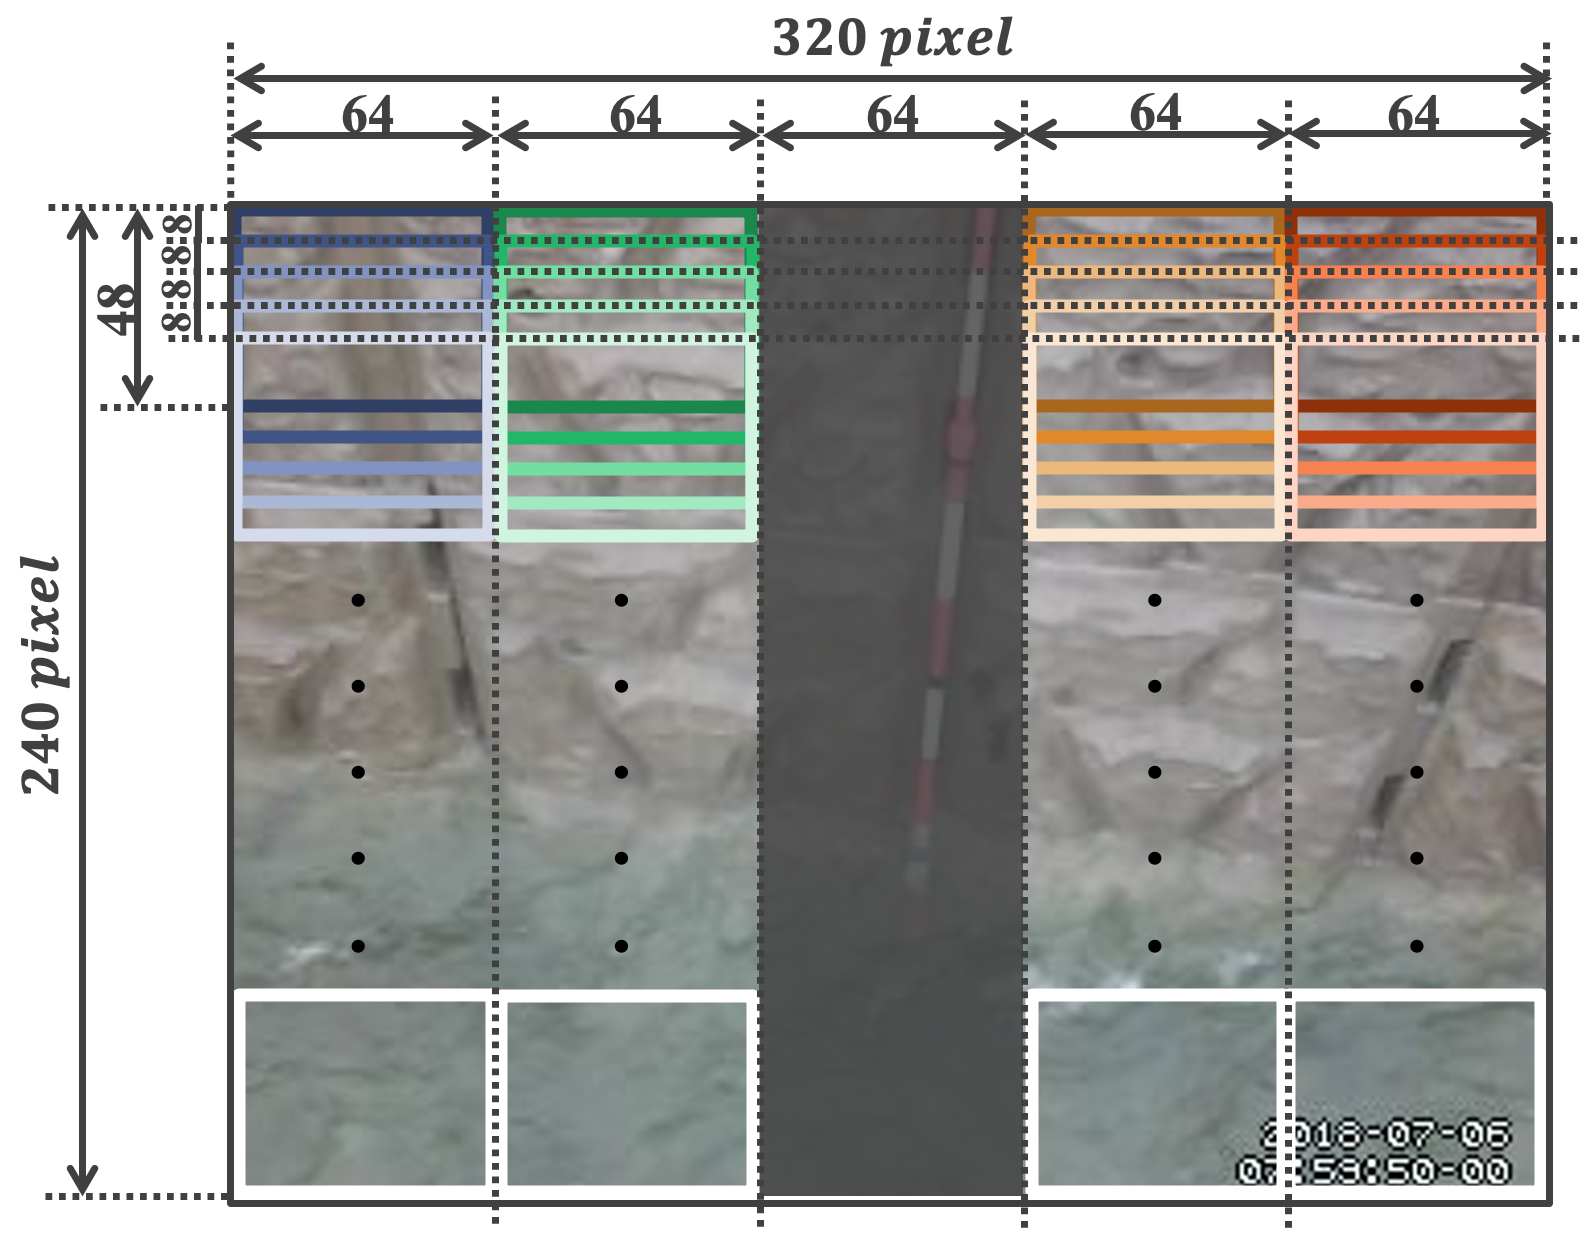
\includegraphics[width=90mm]{figs/kirinuki.png}
  \end{center}
  \caption{切抜画像の生成}
  \label{kirinuki}
\end{figure}

\clearpage
  
\label{3.3}
\subsection{水位の推定方法}
\ref{3.2}節で生成した切り抜き画像を用いて,河川の水位を推定する.各切抜画像に対して
,畳込みニューラルネットワークで学習と分類を行った際に,出力される水面クラスの
ソフトマックス値$S_{water}$と,元画像における縦の座標値$y$を用いて水位の推定を行った.
水位の推定値$E$は元画像から$n$枚の切抜画像が得られたとき以下の式(\ref{e_1})で導出した.
\vspace{5mm}
\begin{equation}
  \label{e_1}
  E=\frac{\sum_{n} y S_{water}}{\sum_{n} S_{water}}
\end{equation}
\vspace{3mm}

例として,水位の推定値を算出する流れを図\ref{suii}で説明する.なお,
説明の際はわかりやすいように,簡略した5列×5枚で切り抜いた場合
について考える.まず,中央の列は測定ポールを含んでいるため除外する.
続いて,各切抜画像を分類し,水面クラスに属する確率に相当する,
ソフトマックス値を算出する(切抜画像内の数値).
また,元の河川の画像における,各切抜画像の上辺と下辺の高さを二分する高さの座標値を求める.
最後に,式(\ref{e_1})に数値を代入することにより,水位の推定値を算出する.
例の場合,水位の推定値 E = 190.8である.このとき,
壁面と水面の境界線は図\ref{suii}の白線の部分であるが,水位の推定値は,
画像中における水面の面積の半分にする縦の座標値に相当する.
例で求めた水位の推定値にしたがって,縦の座標値波線の矢印を引くと,
水面の面積をおよそ半分にする位置に求まっていることが確認できる.
\vspace{3mm}
\begin{figure}[h] 
  \begin{center}
    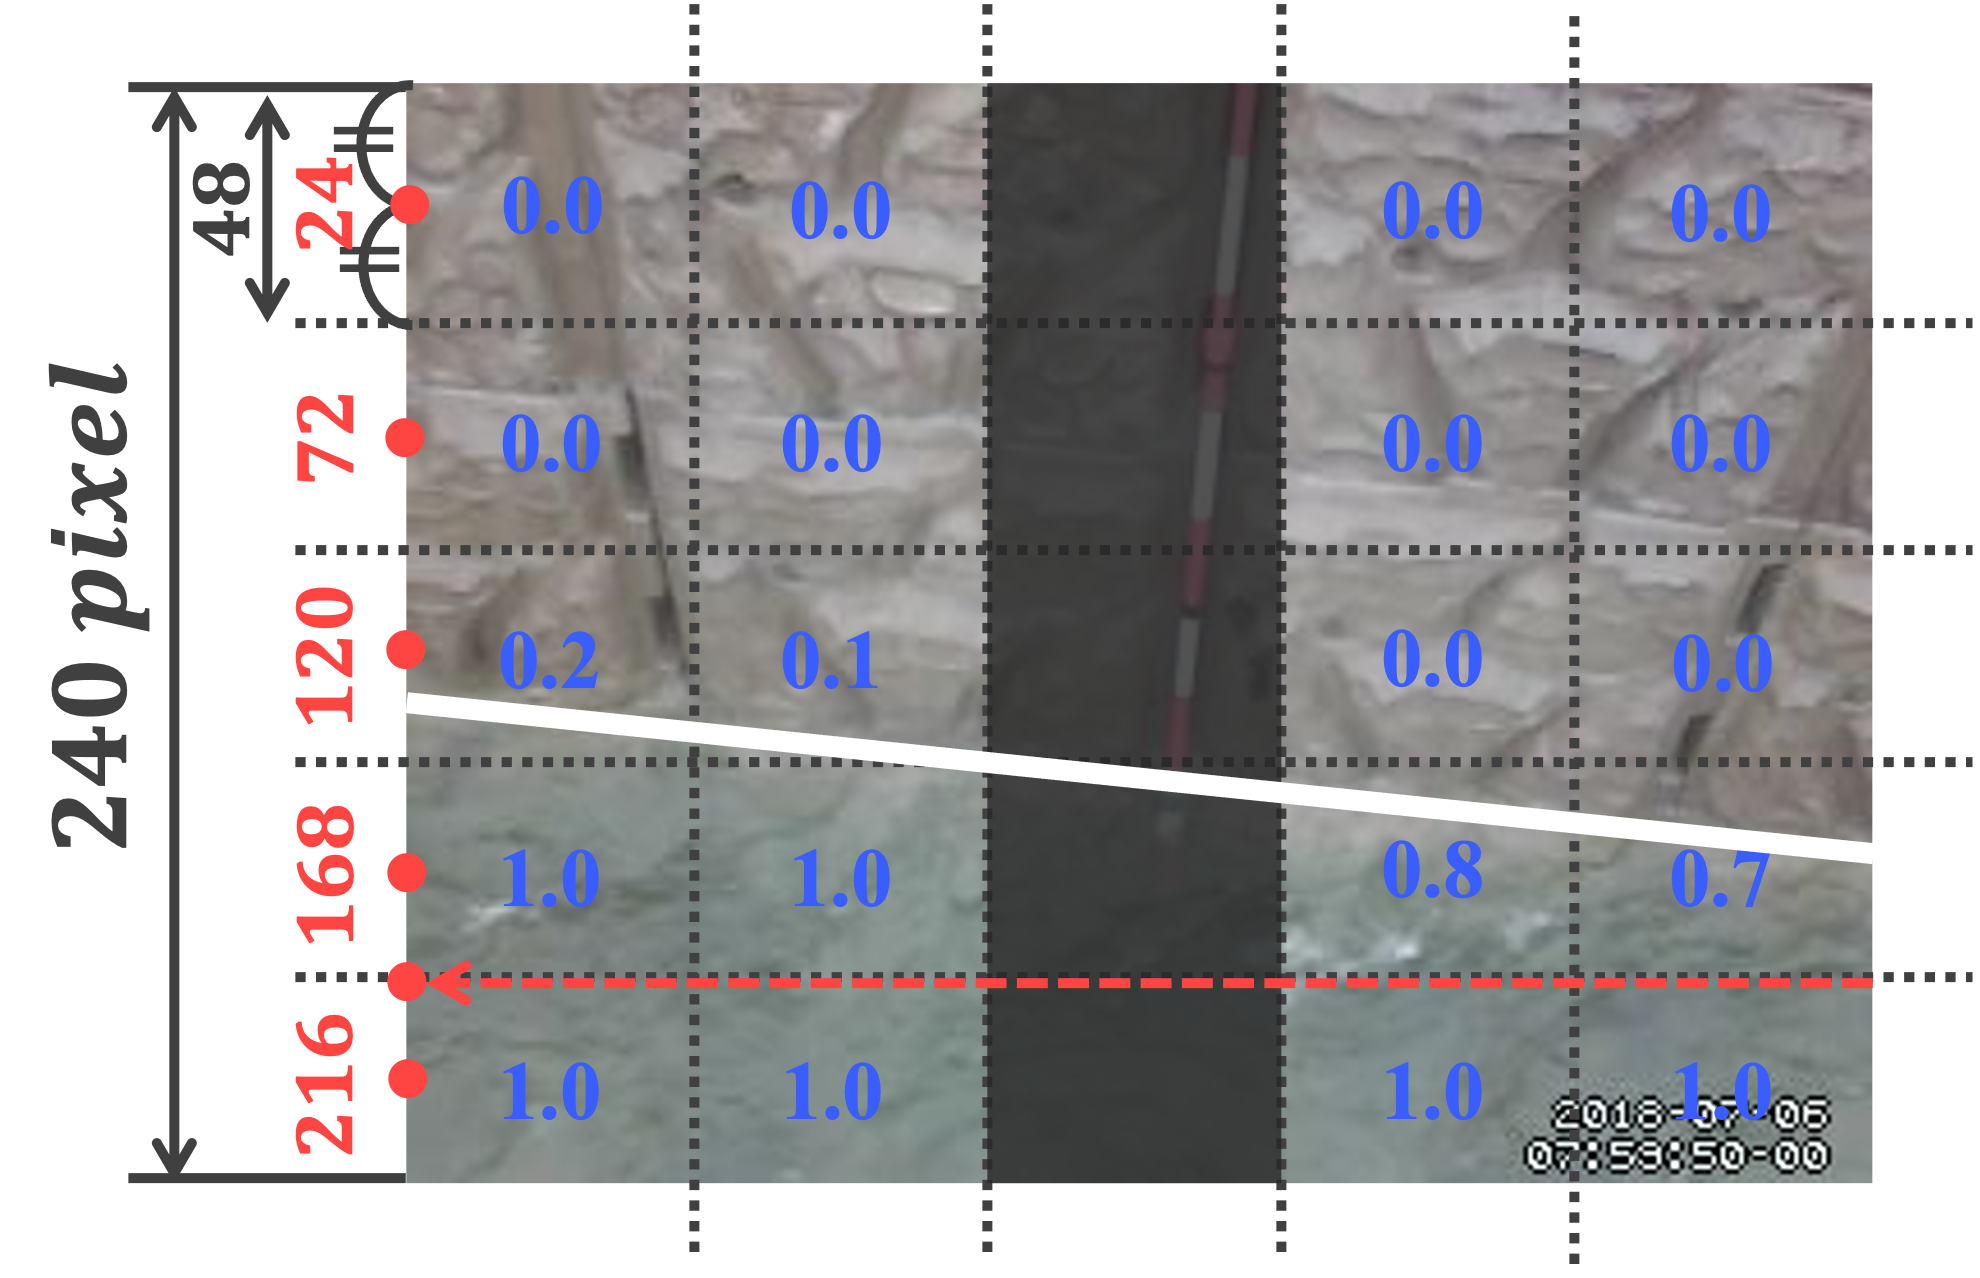
\includegraphics[width=100mm]{figs/suii.png}
    \end{center}
    \caption{推定値算出の流れ}
    \label{suii}
\end{figure}

\clearpage
\subsection{相関係数による評価}
\label{3.4}
式\ref{e_1}によって推定された推定値$E$と,水位計測ポールを参考にして
10分ごとに目視で測定した水位を線形補完した値(測定値)との相関係数を用いて評価した.
\vspace{5mm}
\begin{table}[ht]
  \centering
  \caption{推定値と測定値の相関}  
  \begin{tabular}{rr} \bhline{1.5pt}
     クラス&相関係数 \\ \hline 
   2分類&  0.956\\ \hline
   3分類&  0.930\\ \hline    
  \end{tabular}
  \label{tb:sokan1}
\end{table}
\vspace{5mm}

なお,「水面」「壁面」の2つのクラスで学習と分類を行った
結果を2分類,「水面」「壁面」「その他」の3つのクラスで学習
と分類を行った結果を3分類とした.
\clearpage

%%%%%%%%%%%%%%%%%%%%%%%%%%%%%%%%%%%%%%%%%%%%%%
\section{提案手法}
\subsection{概要}
\label{4.1}
深層学習を用いたセマンティックセグメンテーションでは,
一般的に訓練データとしてアノテーション画像が多数必要であり,アノテーション方法が
精度に影響する.
また,アノテーション画像を手作業で作成する場合,過大な労力がかかる.そこで,本研究では,
可能な労力で必要な精度を達成するための,半自動的なアノテーション方法を提案する.
図\ref{images}に使用した元画像とアノテーション画像の例を示す.

また,抽出結果画像から変換式を用いて水位を推定する方法を提案する.

\vspace{10mm}

\begin{figure}[ht] 
  \begin{center}
    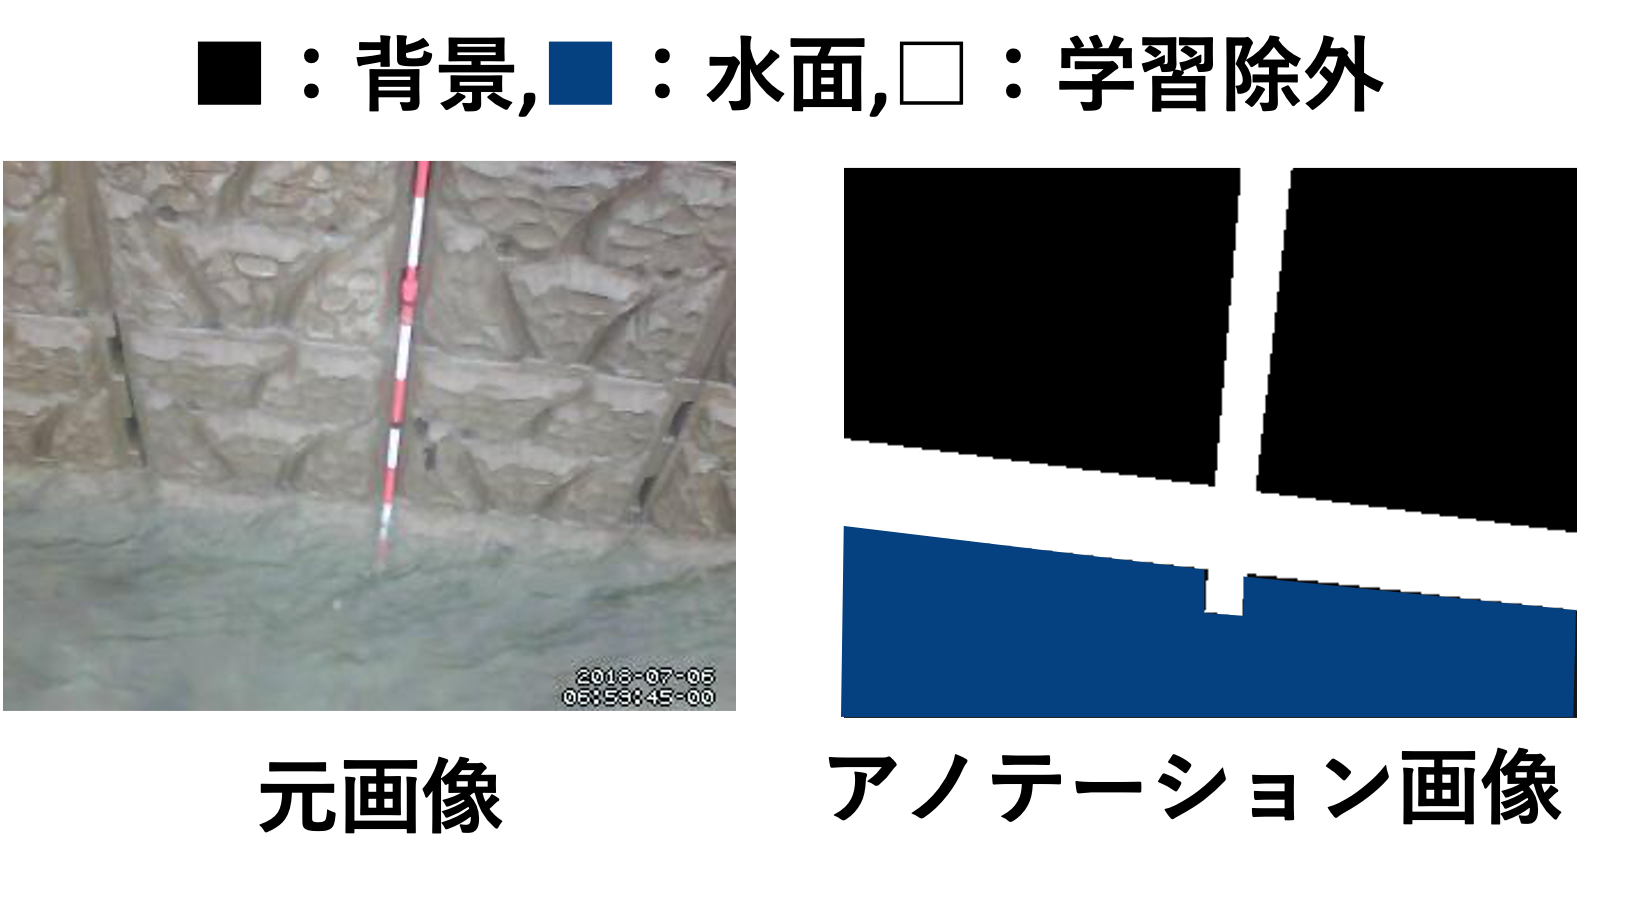
\includegraphics[width=0.8\linewidth]{image/images.png}
  \end{center}
  \vspace{-3mm}
  \caption{元画像とアノテーション画像の例}
  \label{images}
\end{figure}
\clearpage

\subsection{アノテーション方法}
\label{4.2}
本研究で扱った河川の監視カメラ画像には図\ref{image_area}のように「水面」「壁面」「水位計測ポール」「撮影日時」
の4つの範囲がある.従って,本研究では以下の方法によってアノテーション画像を
作成した.
\begin{description}
  \item・図\ref{area}のように
  「水面」と「壁面」の範囲は水位によって変化するため,目視
  によって10分毎の水位を推定し,その測定値から線形補間によって自動的に範囲を
  決定した.
  \vspace{-3mm}
  \item・確実なラベル付けを行うため,図\ref{aimai}のような
  「水面」と「壁面」の境界が曖昧な範囲を学習対象から除外した.
  除外範囲決定の流れを図\ref{ano2}に示す.
  \vspace{-3mm}
  \item・「水位計測ポール」と「撮影日時」の範囲は図\ref{day_pole}のように
  時間によらず変化しないため,目視で決定した.
\end{description}.

\begin{figure}[ht]
  \centering
  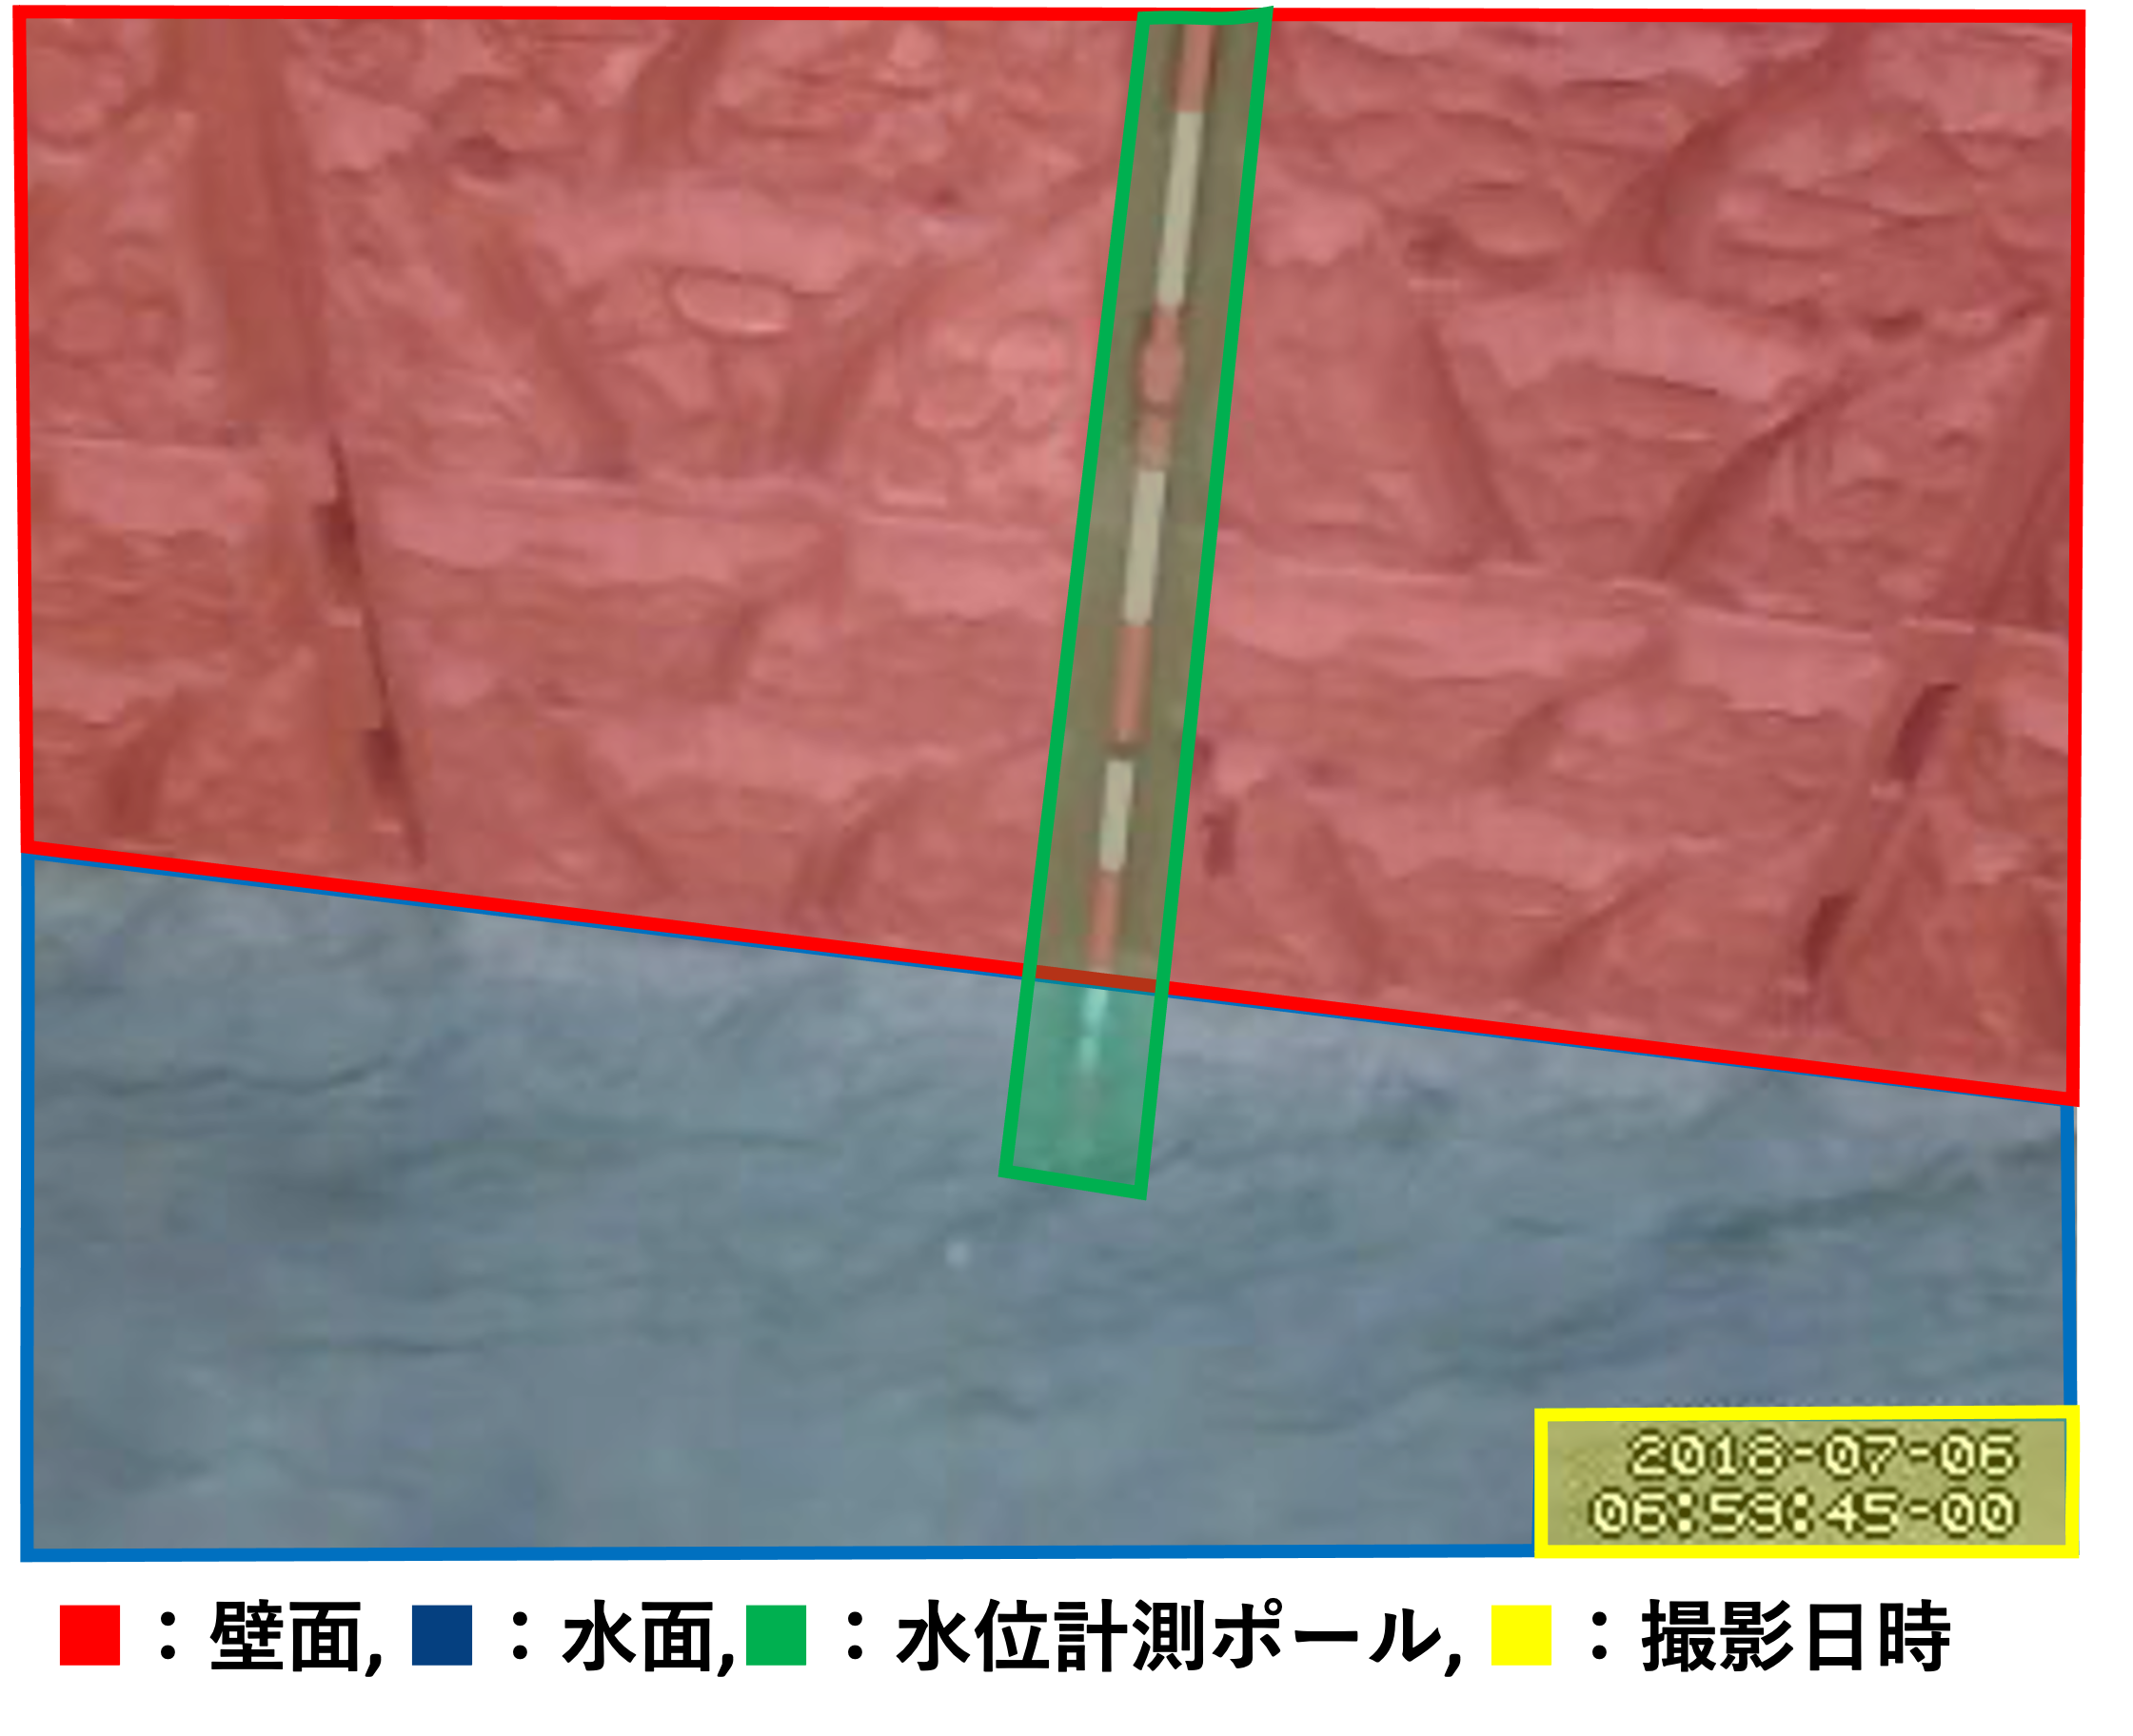
\includegraphics[keepaspectratio,width=0.8\linewidth]{image/image_area.png}
  \caption{4つの範囲}
  \label{image_area}
\end{figure}

\begin{figure}[ht]
  \centering
  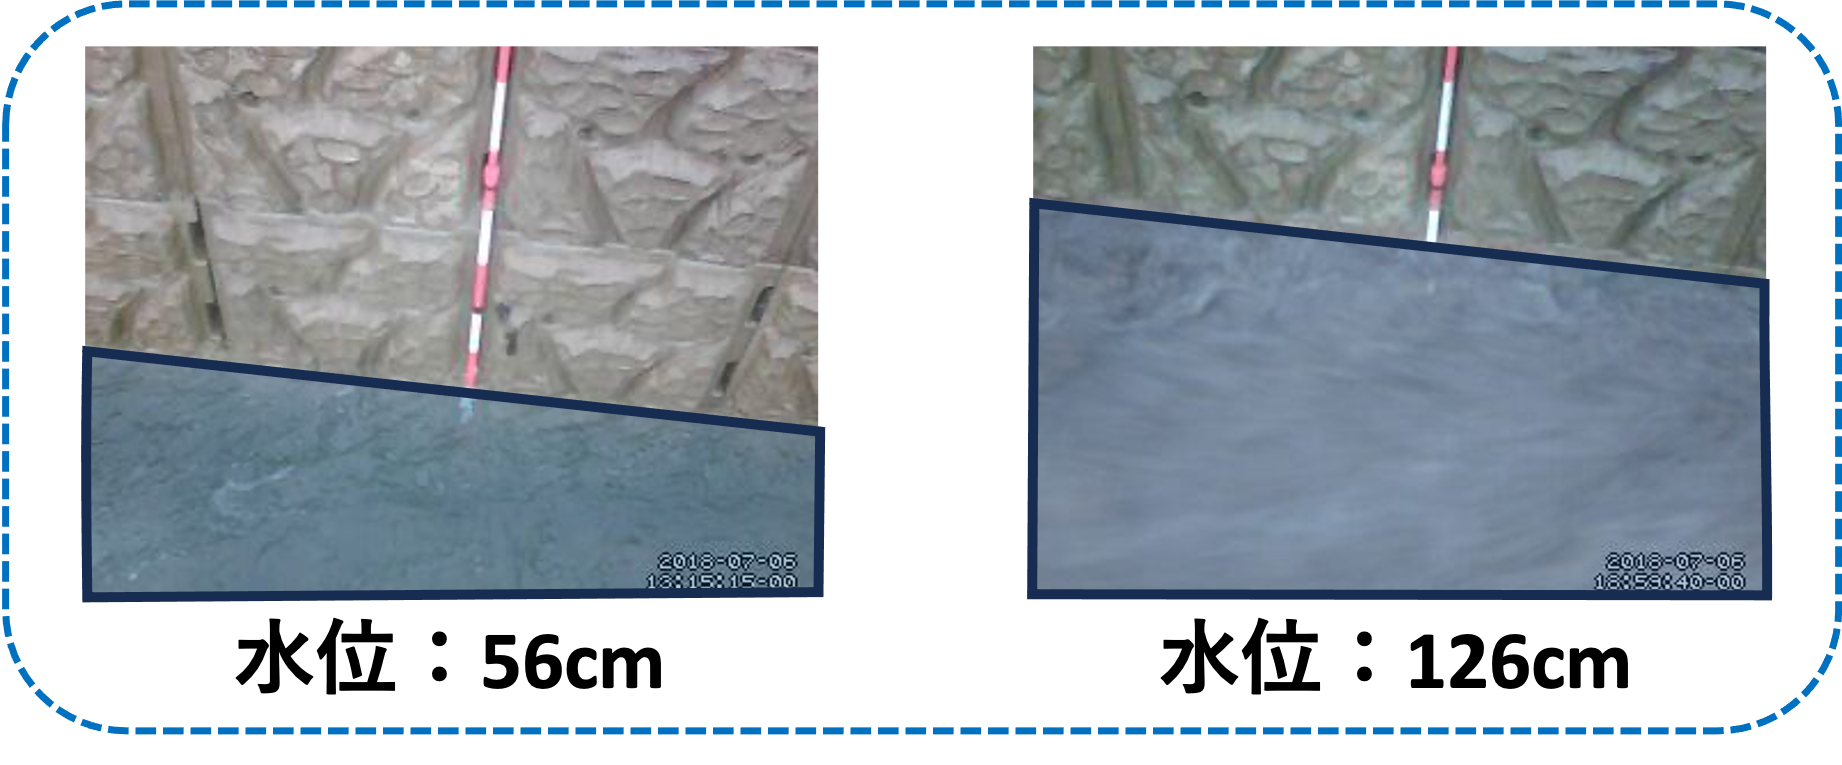
\includegraphics[keepaspectratio,width=0.9\linewidth]{image/water_level.png}
  \caption{水位による範囲の変化}
  \label{area}
\end{figure}

\begin{figure}[ht]
  \centering
  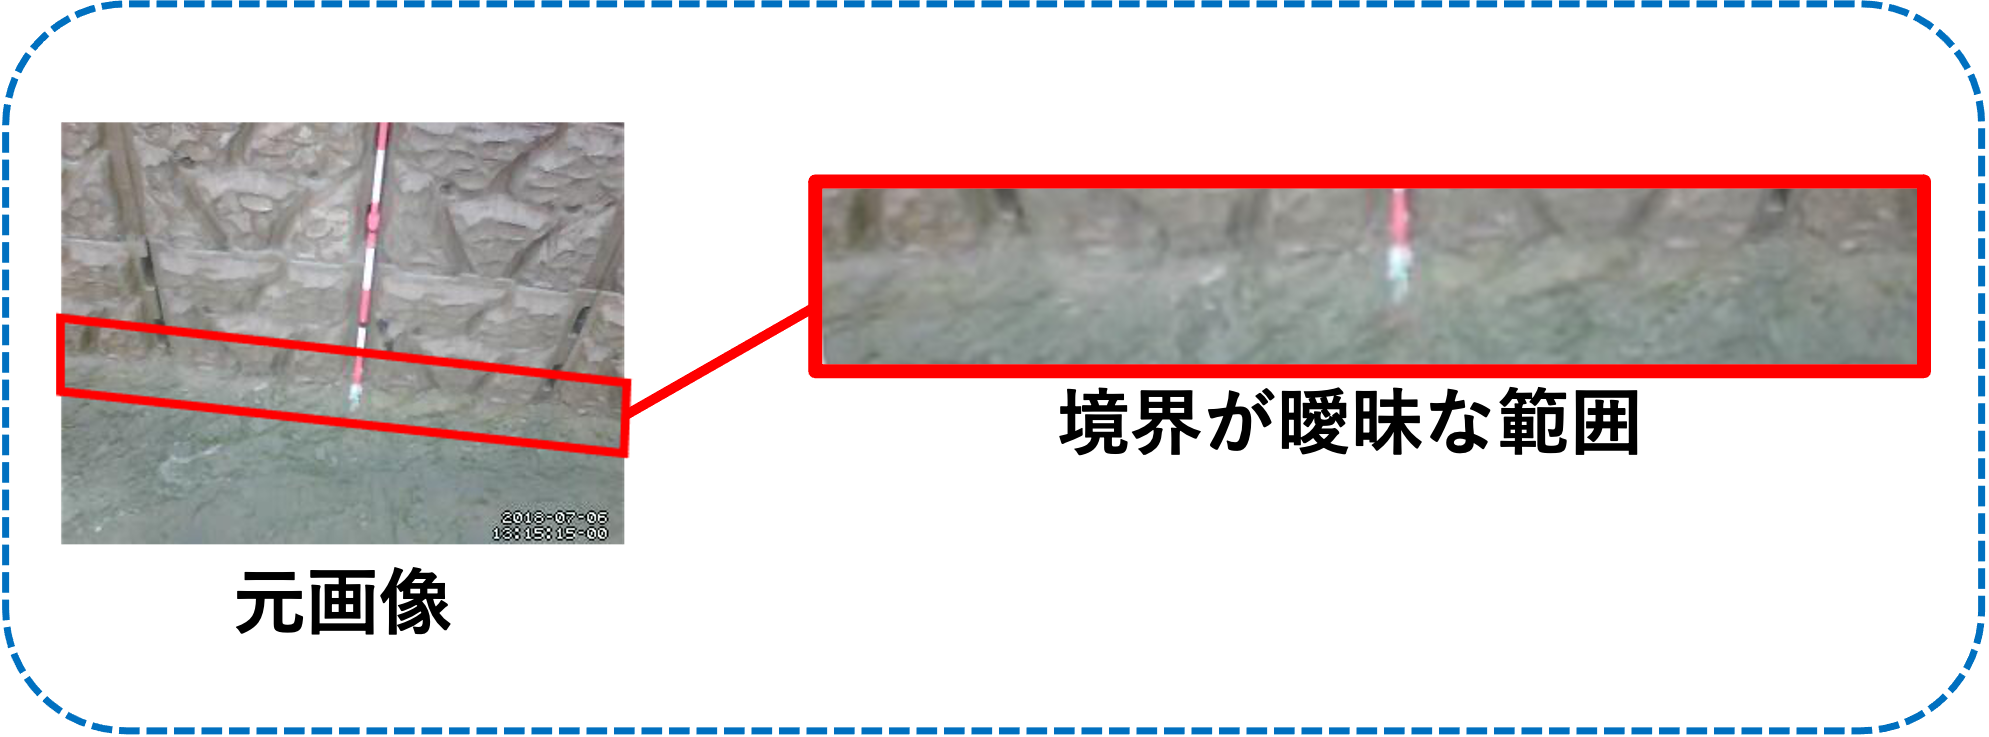
\includegraphics[keepaspectratio,width=0.9\linewidth]{image/aimai.png}
  \caption{「水面」と「壁面」の境界が曖昧な範囲}
  \label{aimai}
\end{figure}

\begin{figure}[ht]
  \centering
  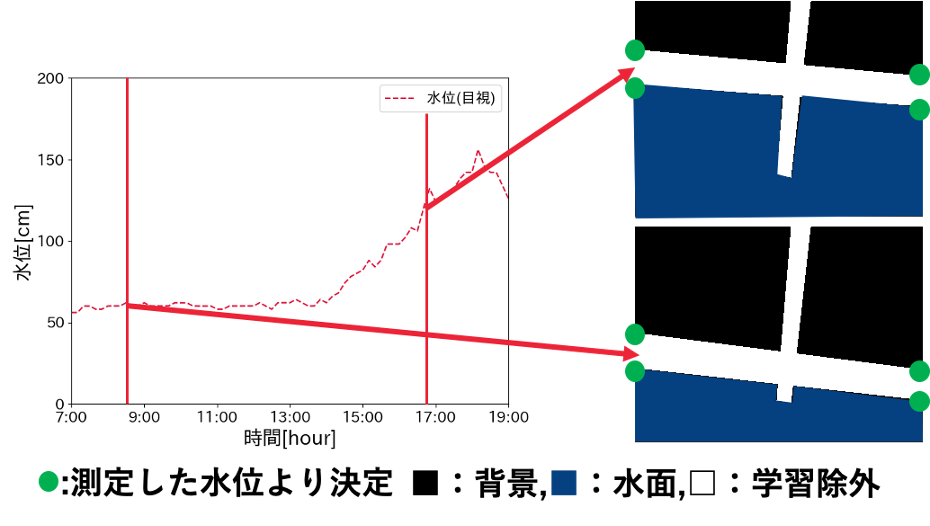
\includegraphics[keepaspectratio,width=0.8\linewidth]{image/ano2.png}
  \caption{範囲決定の流れ}
  \label{ano2}
\end{figure}

\begin{figure}[t]
  \centering
  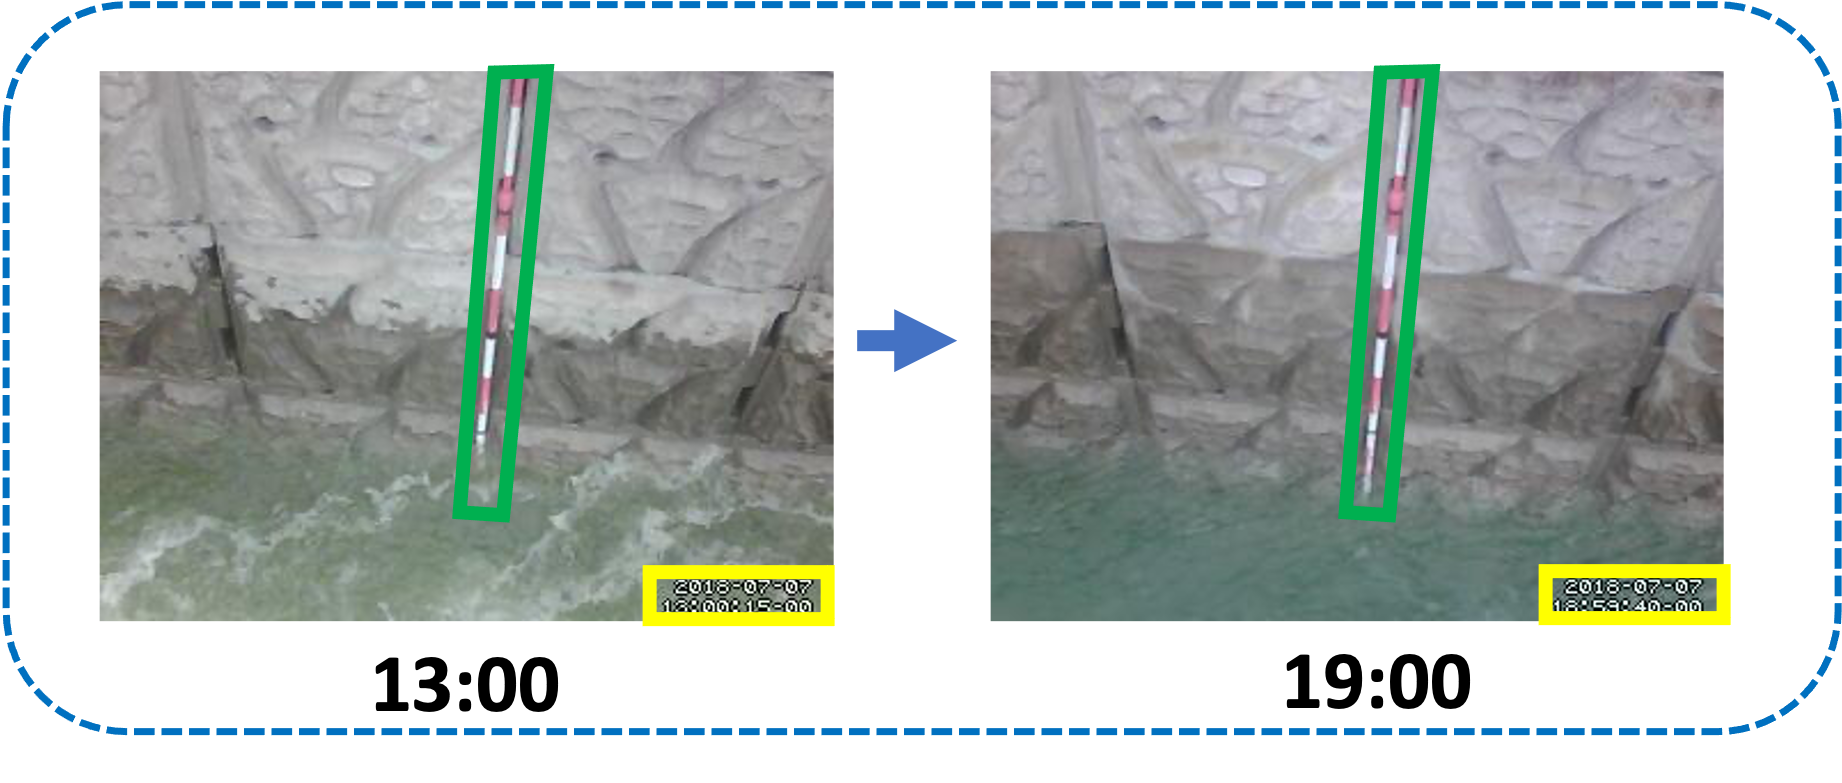
\includegraphics[keepaspectratio,width=0.9\linewidth]{image/day_pole.png}
  \caption{「水位計測ポール」と「撮影日時」の範囲}
  \label{day_pole}
\end{figure}

\clearpage


\subsection{水位の推定方法}
\label{4.3}
画像内の水面領域の面積割合と水位の散布図を図\ref{soukan}に示す.
また,水面領域の面積割合と水位の相関係数は0.99となった.
従って,水面領域の面積割合から水位へ値を変換する式(\ref{change})を作成した.
この変換式を使用して,図\ref{pre_image}に示す領域抽出結果画像から取得した水面領域の面積割合を
水位の推定値へ変換した.

\begin{equation}
  \label{change}
  \mbox{水位} =  243.78×\mbox{水面領域の面積割合}-23.23
\end{equation}

\begin{figure}[ht] 
  \begin{center}
    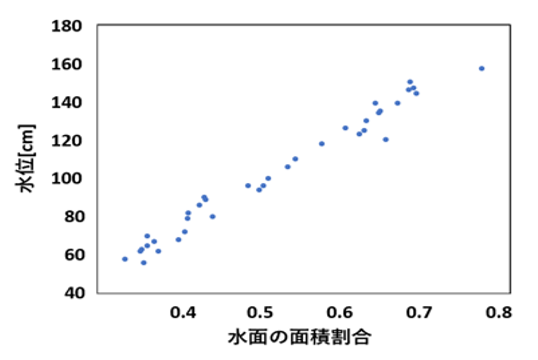
\includegraphics[width=0.7\linewidth]{image/soukan.png}
  \end{center}
  \caption{水面領域の面積割合と水位の散布図}
  \label{soukan}
\end{figure}

\vspace{5mm}

\begin{figure}[ht] 
  \begin{center}
    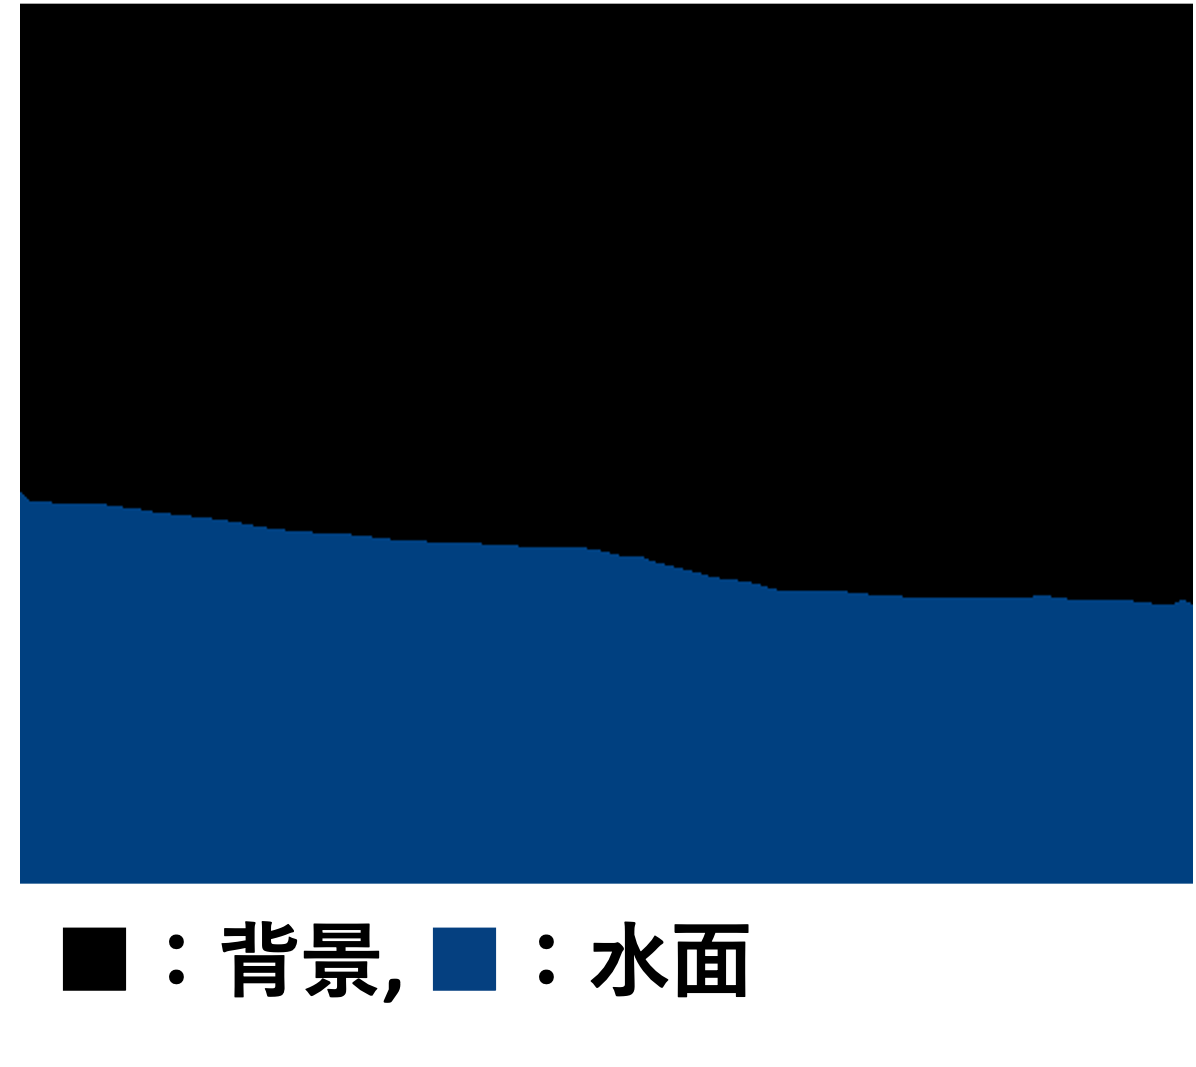
\includegraphics[width=0.5\linewidth]{image/pre_image.png}
  \end{center}
  \caption{領域抽出結果画像}
  \label{pre_image}
\end{figure}


\clearpage
%%%%%%%%%%%%%%%%%%%%%%%%%%%%%%%%%%%%%%%%%%%%%%
\section{評価実験}
目視で計測した水位とSS手法を用いて推定した水位のRMSE(Root Mean Square Error)
を先行研究\cite{watanabe}で比較することにより,SS手法の評価を行う.
また,提案したアノテーション方法で作成したモデルの領域抽出精度を評価することにより
提案手法の有効性を示す.

本研究では河川画像として,本学情報工学科モニタリングネットワーク研究室にて
運用中の広島市安佐北区三入地区桐原川の監視システムにおいて撮影された
図\ref{togegawa}の監視カメラ画像を使用した.
また,畳込みニューラルネットワークによるセマンティックセグメンテーションのシステムとして,
DeepLabv3+\cite{deeplabv3+}を用いた.

\vspace{5mm}
\begin{figure}[h] 
  \begin{center}
    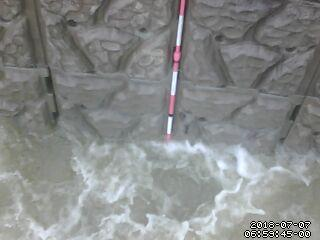
\includegraphics[width=0.8\linewidth]{image/070001.jpg}
  \end{center}
  \caption{桐原川の監視カメラ画像}
  \label{togegawa}
\end{figure}
\clearpage

領域抽出結果についての評価は,IoU(Interaction over Union)\cite{IoU}
とF値\cite{bf}を用いて行う.
IoUは図\ref{tp}と式(\ref{IoU})で定義される予測領域と正解領域の
オーバーラップ率を意味する値である.

F値は図\ref{tp}と式(\ref{Recall}),(\ref{Precision}),(\ref{F score}),
で表される値である.感度は正解画像の中で水面領域であ
る画素数に対して,予測結果においても水面領域と判定
した割合である.また,適合率は予測結果の中で水面領域
と判定した画素数について,正解画像においても
水面領域である割合である.そして,F値は一般にトレードオフの関係
になる感度と適合率の両方を評価する.
今回はすべての画像に対する水面クラスの平均IoUと平均F値に
着目して評価を行う.
\vspace{5mm}
\begin{figure}[ht] 
  \begin{center}
    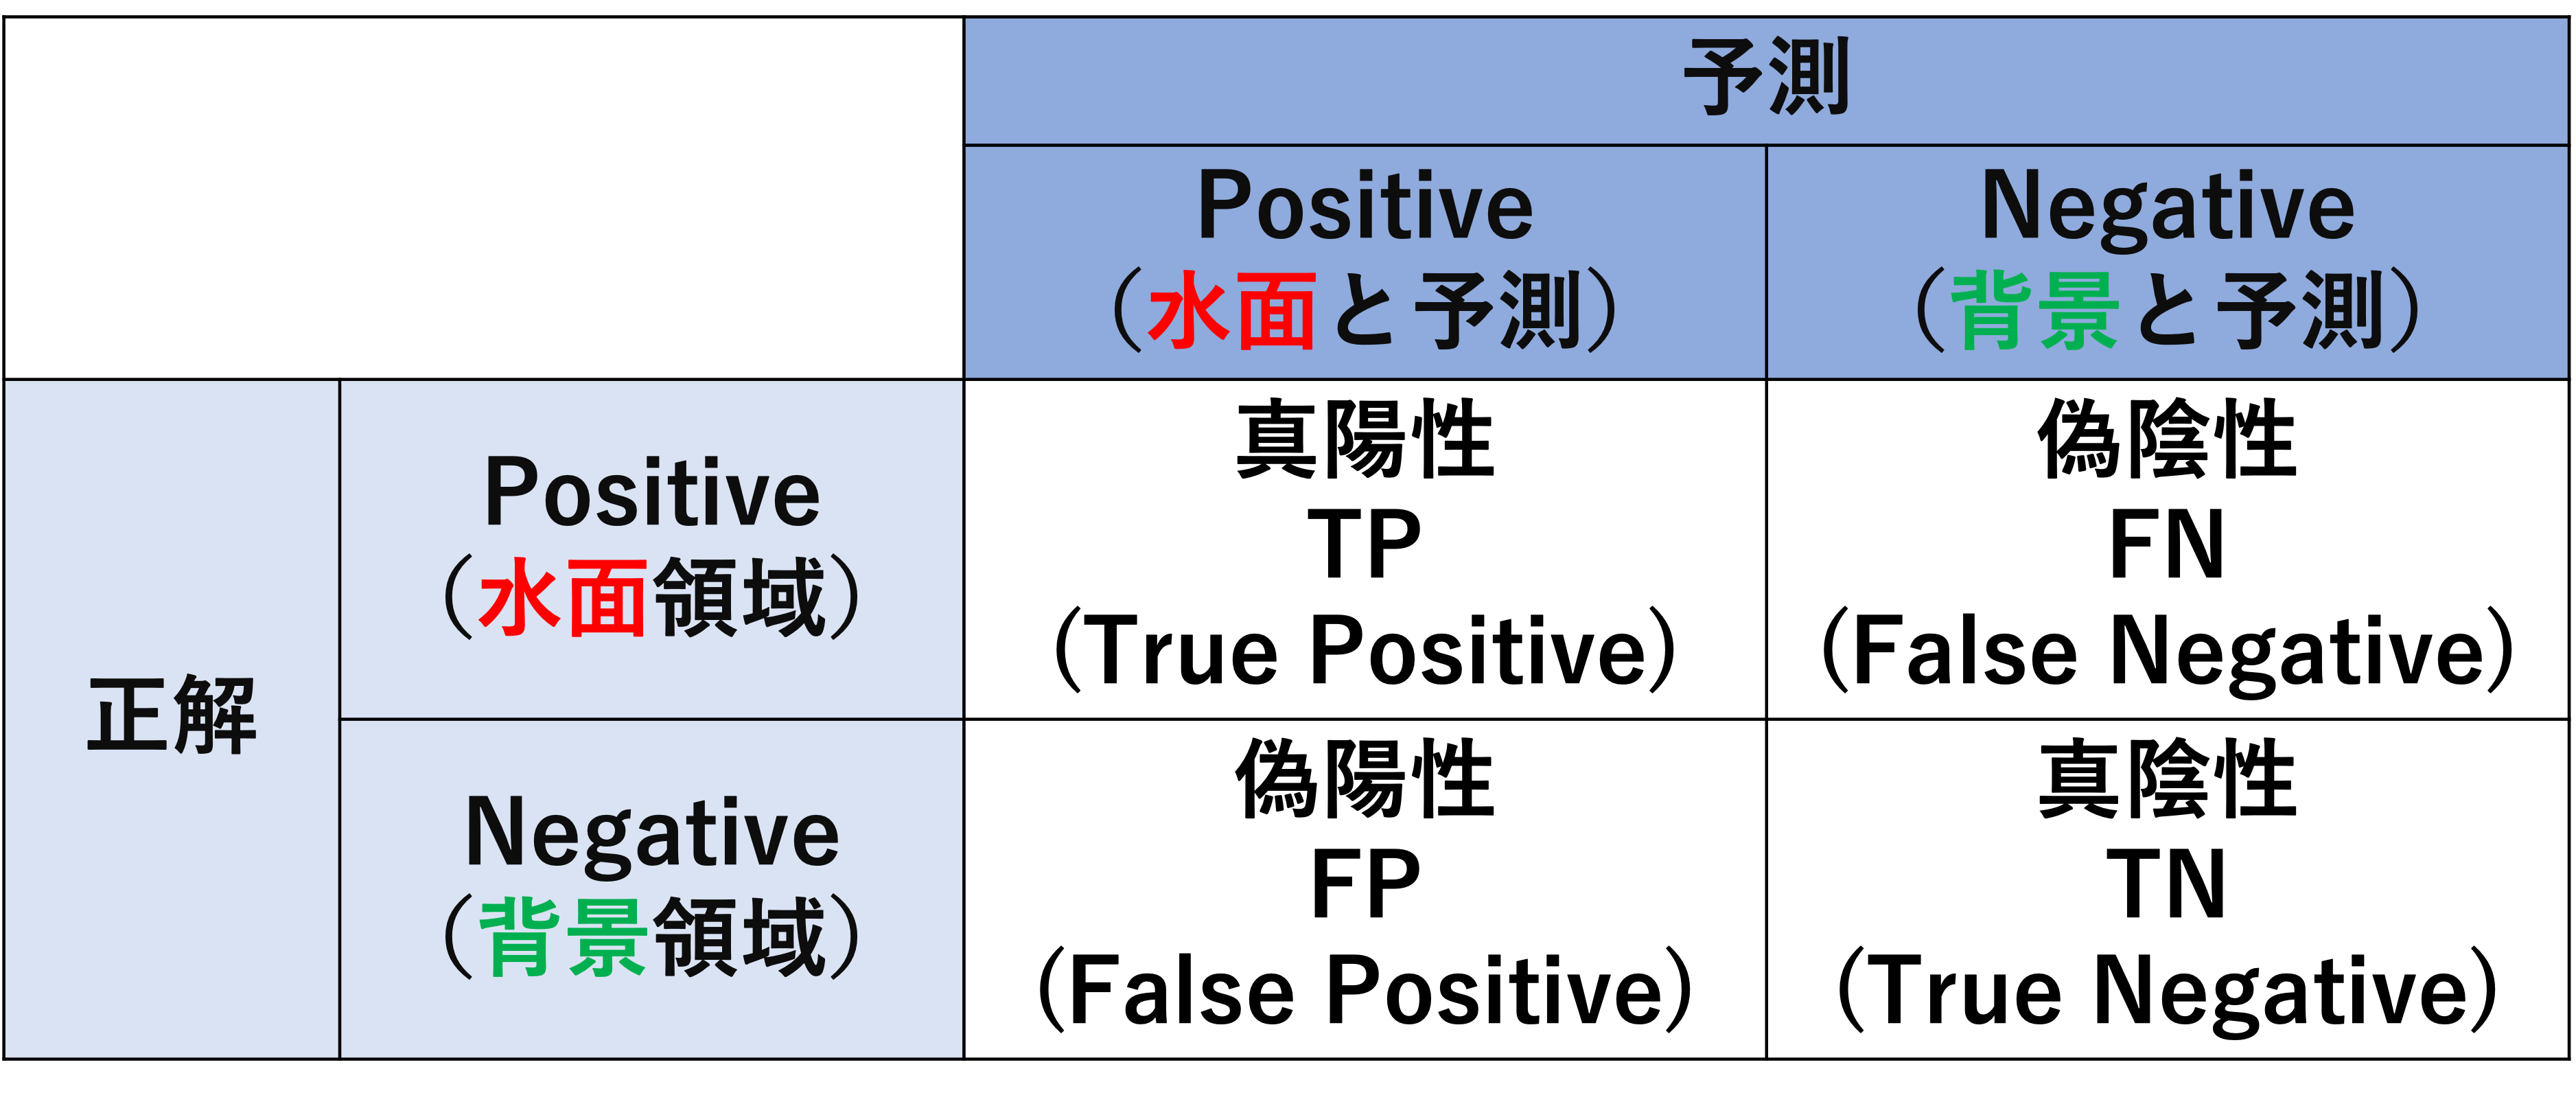
\includegraphics[width=0.8\linewidth]{image/TP.png}
  \end{center}
  \caption{領域抽出における分類問題の混合行列の定義}
  \label{tp}
\end{figure}

\begin{equation}
  \label{IoU}
  \mbox{IoU} =  \frac{\mbox{TP}}{\mbox{TP}+\mbox{FP}+\mbox{FN}}
\end{equation}

\begin{equation}
  \label{Recall}
  \mbox{感度} =  \frac{\mbox{TP}}{\mbox{TP}+\mbox{FN}}
\end{equation}

\begin{equation}
  \label{Precision}
  \mbox{適合率} =  \frac{\mbox{TP}}{\mbox{TP}+\mbox{FP}}
\end{equation}

\begin{equation}
  \label{F score}
  \mbox{F値} =  2×\frac{\mbox{適合率}×\mbox{感度}}{\mbox{適合率}+\mbox{感度}}
\end{equation}
\vspace{5mm}
\clearpage

\subsection{学習モデルの構築と評価}
\label{5.1}
セマンティックセグメンテーションモデルの
学習回数を変化させて領域抽出を行い,その結果を
IoUとF値を利用して評価することにより,モデルの適切な学習回数の調査を行った.
学習回数を50,100,200,300...,1000と変化させて
セマンティックセグメンテーションモデルを作成した.
また,2018年7月6日の7:00から19:00までの画像を訓練データ(8147枚)に,
テストデータには同年の7月7日同時間帯の画像データ(8086枚)を用いた.

作成したモデルを用いて領域抽出を行い,学習回数毎にIoUとF値を求めた.
図\ref{learn}はモデルの学習回数と抽出精度の関係を表したグラフである.

\begin{figure}[ht] 
  \begin{center}
    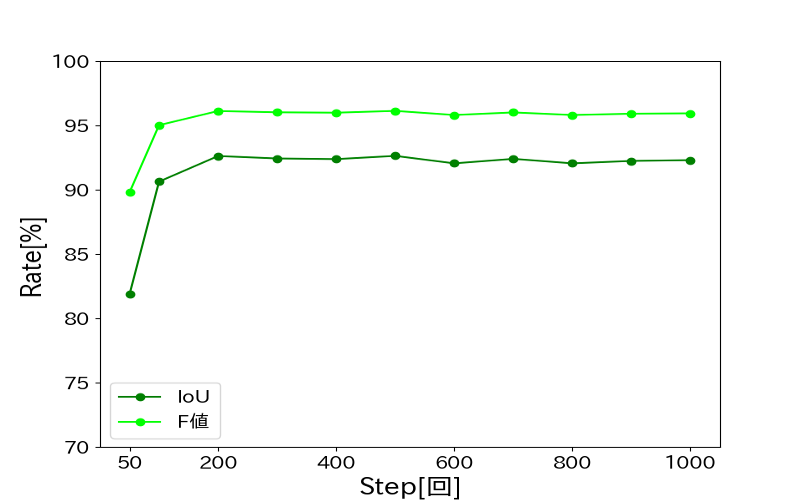
\includegraphics[width=150mm]{image/Step_IoU_F.png}
  \end{center}
  \caption{学習回数とIoU,F値の関係}
  \label{learn}
\end{figure}
\clearpage

\subsection{ラベル設定と評価}
\label{5.2}

2種類のアノテーション設定で構築したモデルの領域抽出精度を
IoUとF値で比較することにより,水位計測ポールに対する適切なラベル設定の調査を行う.
設定Aと設定Bの二つの設定でアノテーションを行った.
図\ref{anoAB}で示すように,
設定Aは水面と撮影日時に水面ラベル,壁面に背景ラベル,水位計測ポールを学習除外領域に設定した.
また,設定Bは水位計測ポール以外は設定Aと統一し,水位計測ポールに水位計測ポールラベルを与えた.
訓練データとテストデータには\ref{5.1}節と同じデータを使用した.

\begin{figure}[ht] 
  \begin{center}
    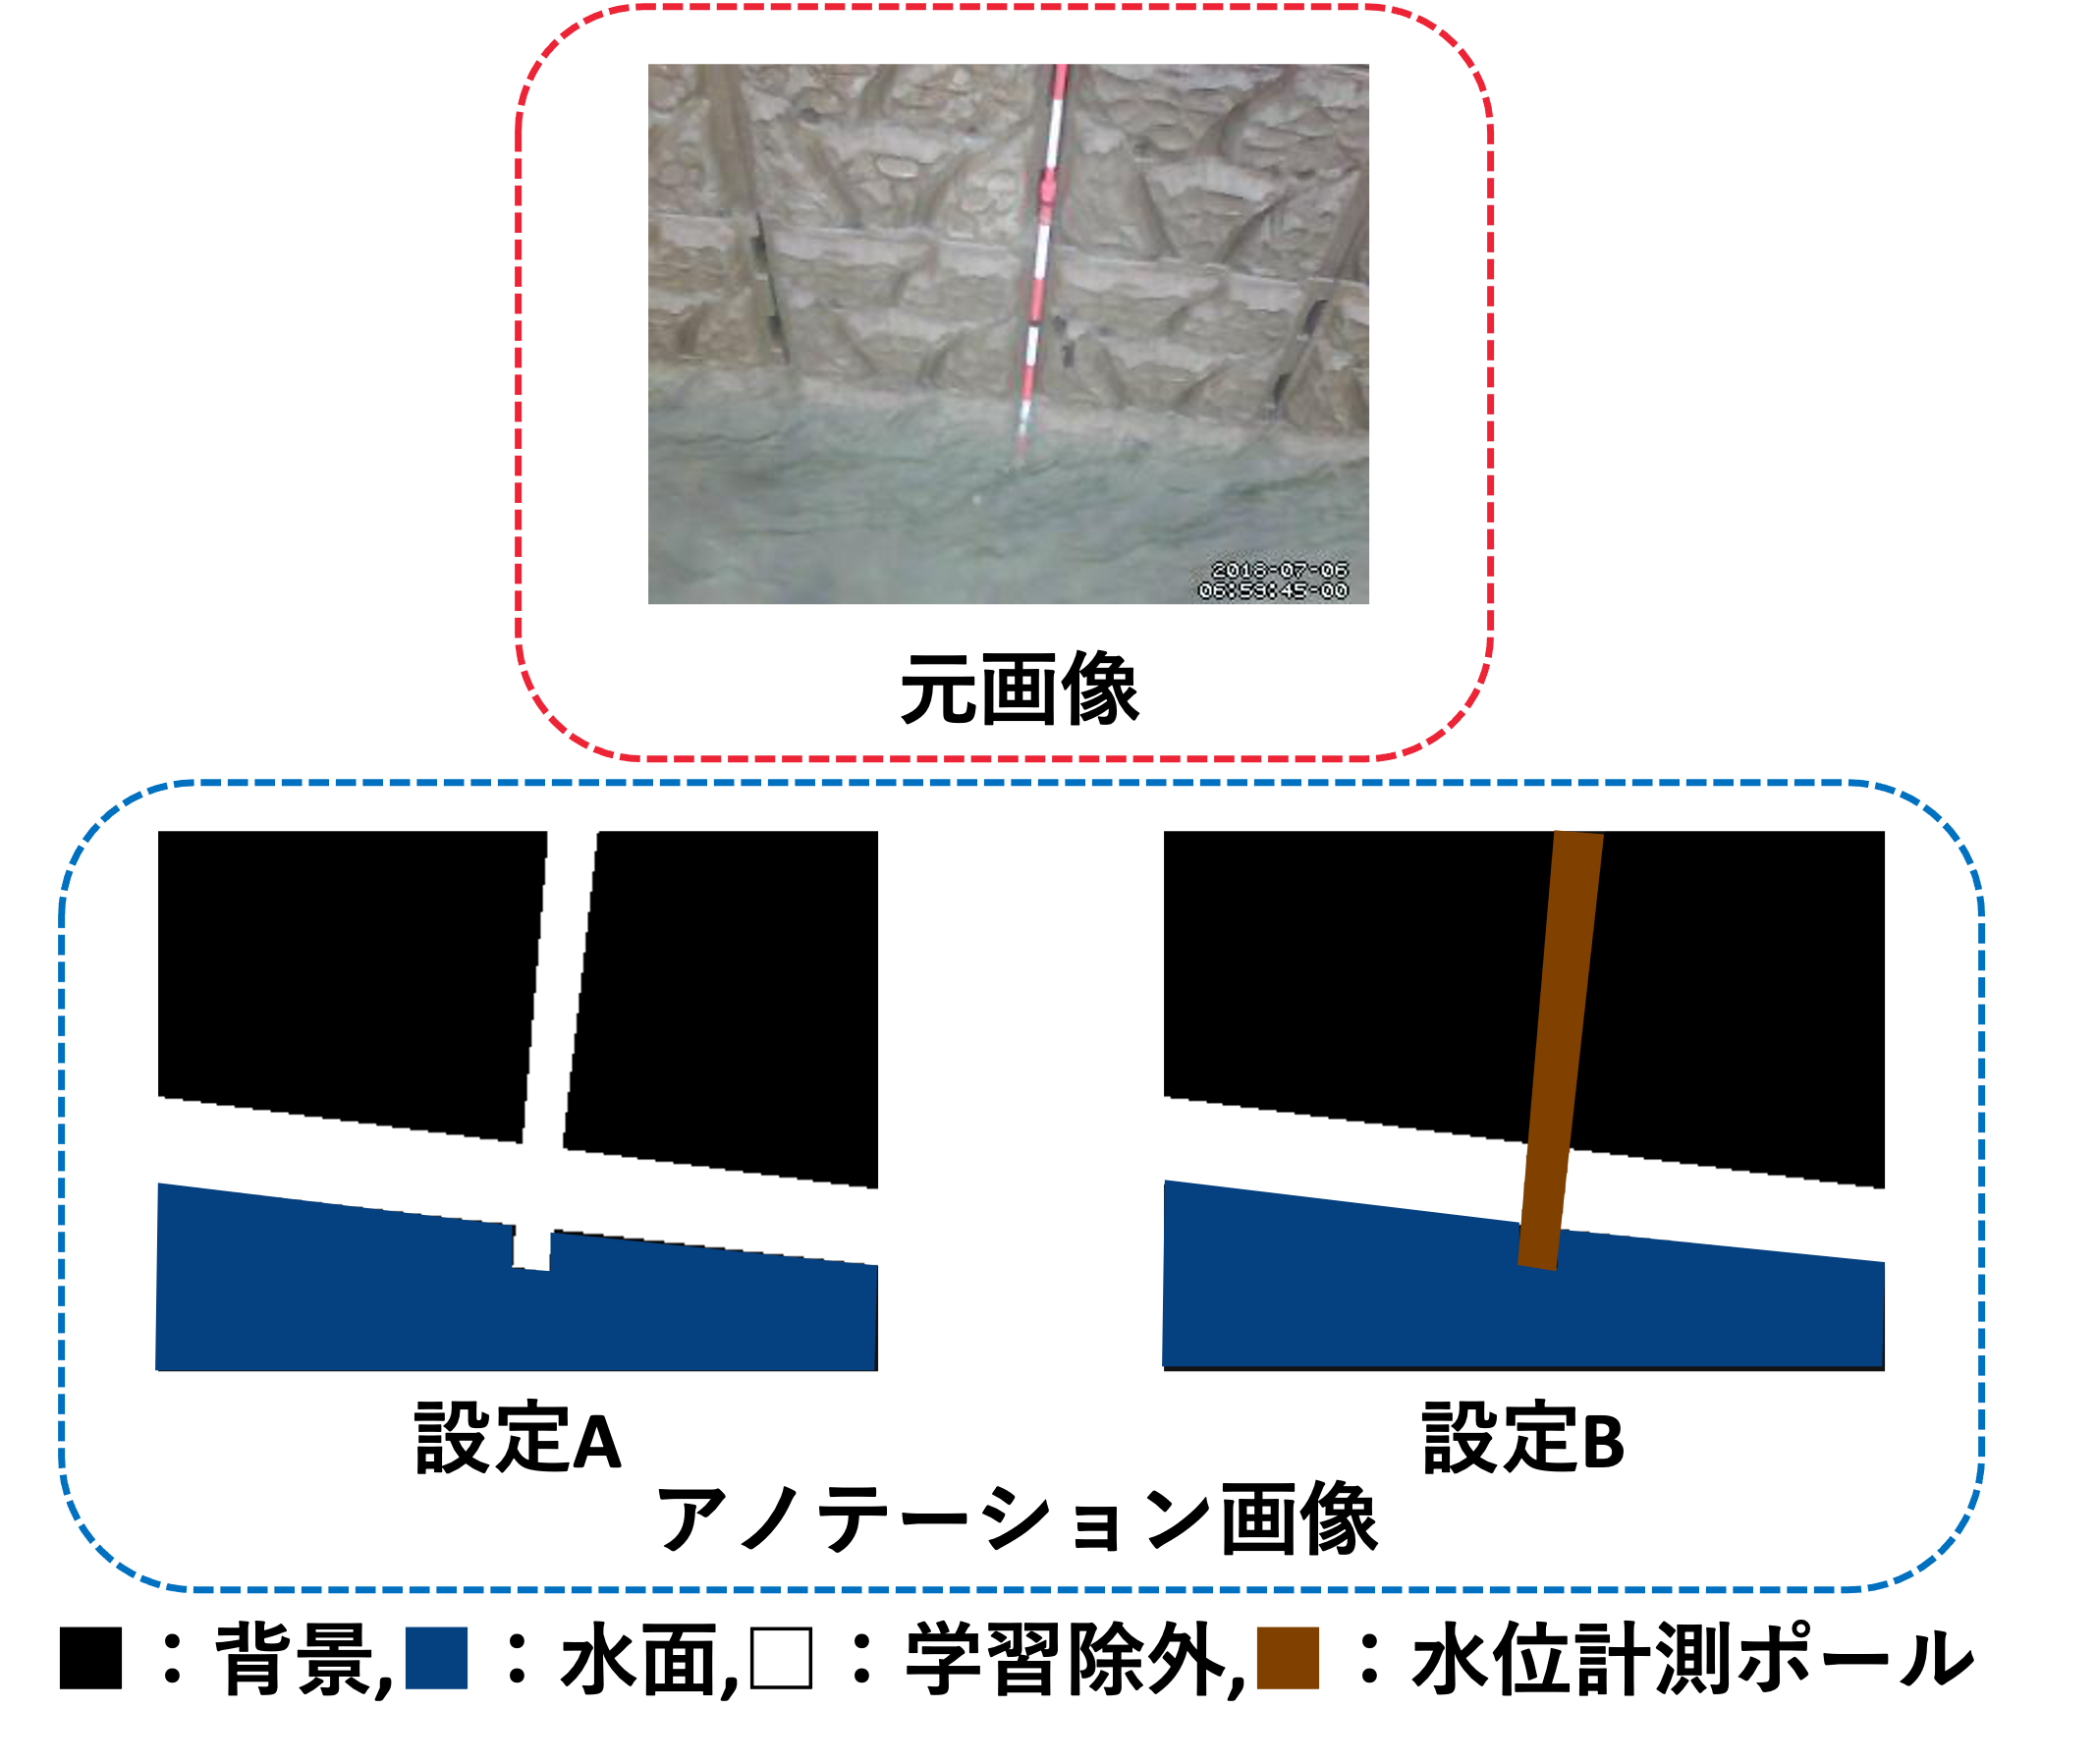
\includegraphics[width=0.8\linewidth]{image/anoAB.png}
  \end{center}
  
  \caption{アノテーション画像例}
  \label{anoAB}
\end{figure}
\vspace{3mm}

それぞれの設定のIoUとF値は表\ref{pole}の通りとなった. 
また,時間別のIoUを図\ref{AB_IoU}に,
時間別のF値の値を図\ref{AB_bf}に示す.
それぞれのモデルの抽出結果例を図\ref{AB_image}に示す.

\begin{table}[ht]
  \centering
  \caption{IoU(%)とF値(%)}  
  \begin{tabular}{lrr} \bhline{1.5pt}
     &IoU&F値\\ \hline 
   設定A&92.30& 95.94\\ \hline  
   設定B&88.57&  93.89\\ \hline  
  \end{tabular}
  \label{pole}
\end{table}

\begin{figure}[ht] 
  \begin{center}
    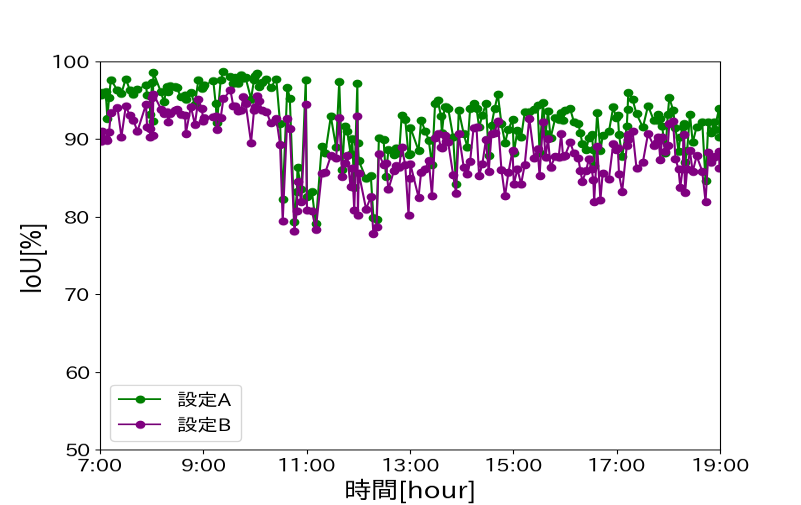
\includegraphics[width=\linewidth]{image/0707_AB_IoU.png}
  \end{center}
  \caption{時間別IoU}
  \label{AB_IoU}
\end{figure}

\begin{figure}[ht] 
  \begin{center}
    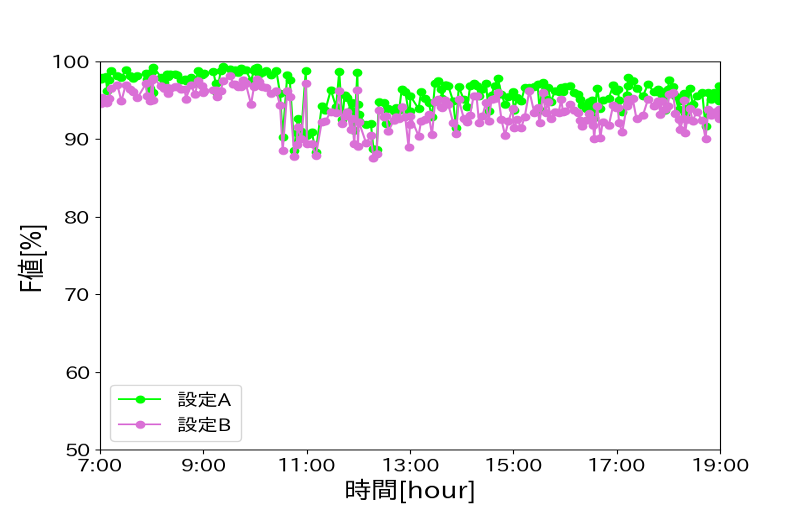
\includegraphics[width=\linewidth]{image/0707_AB_bf.png}
  \end{center}
  \caption{時間別F値}
  \label{AB_bf}
\end{figure}
\clearpage

\begin{figure}[t] 
  \begin{center}
    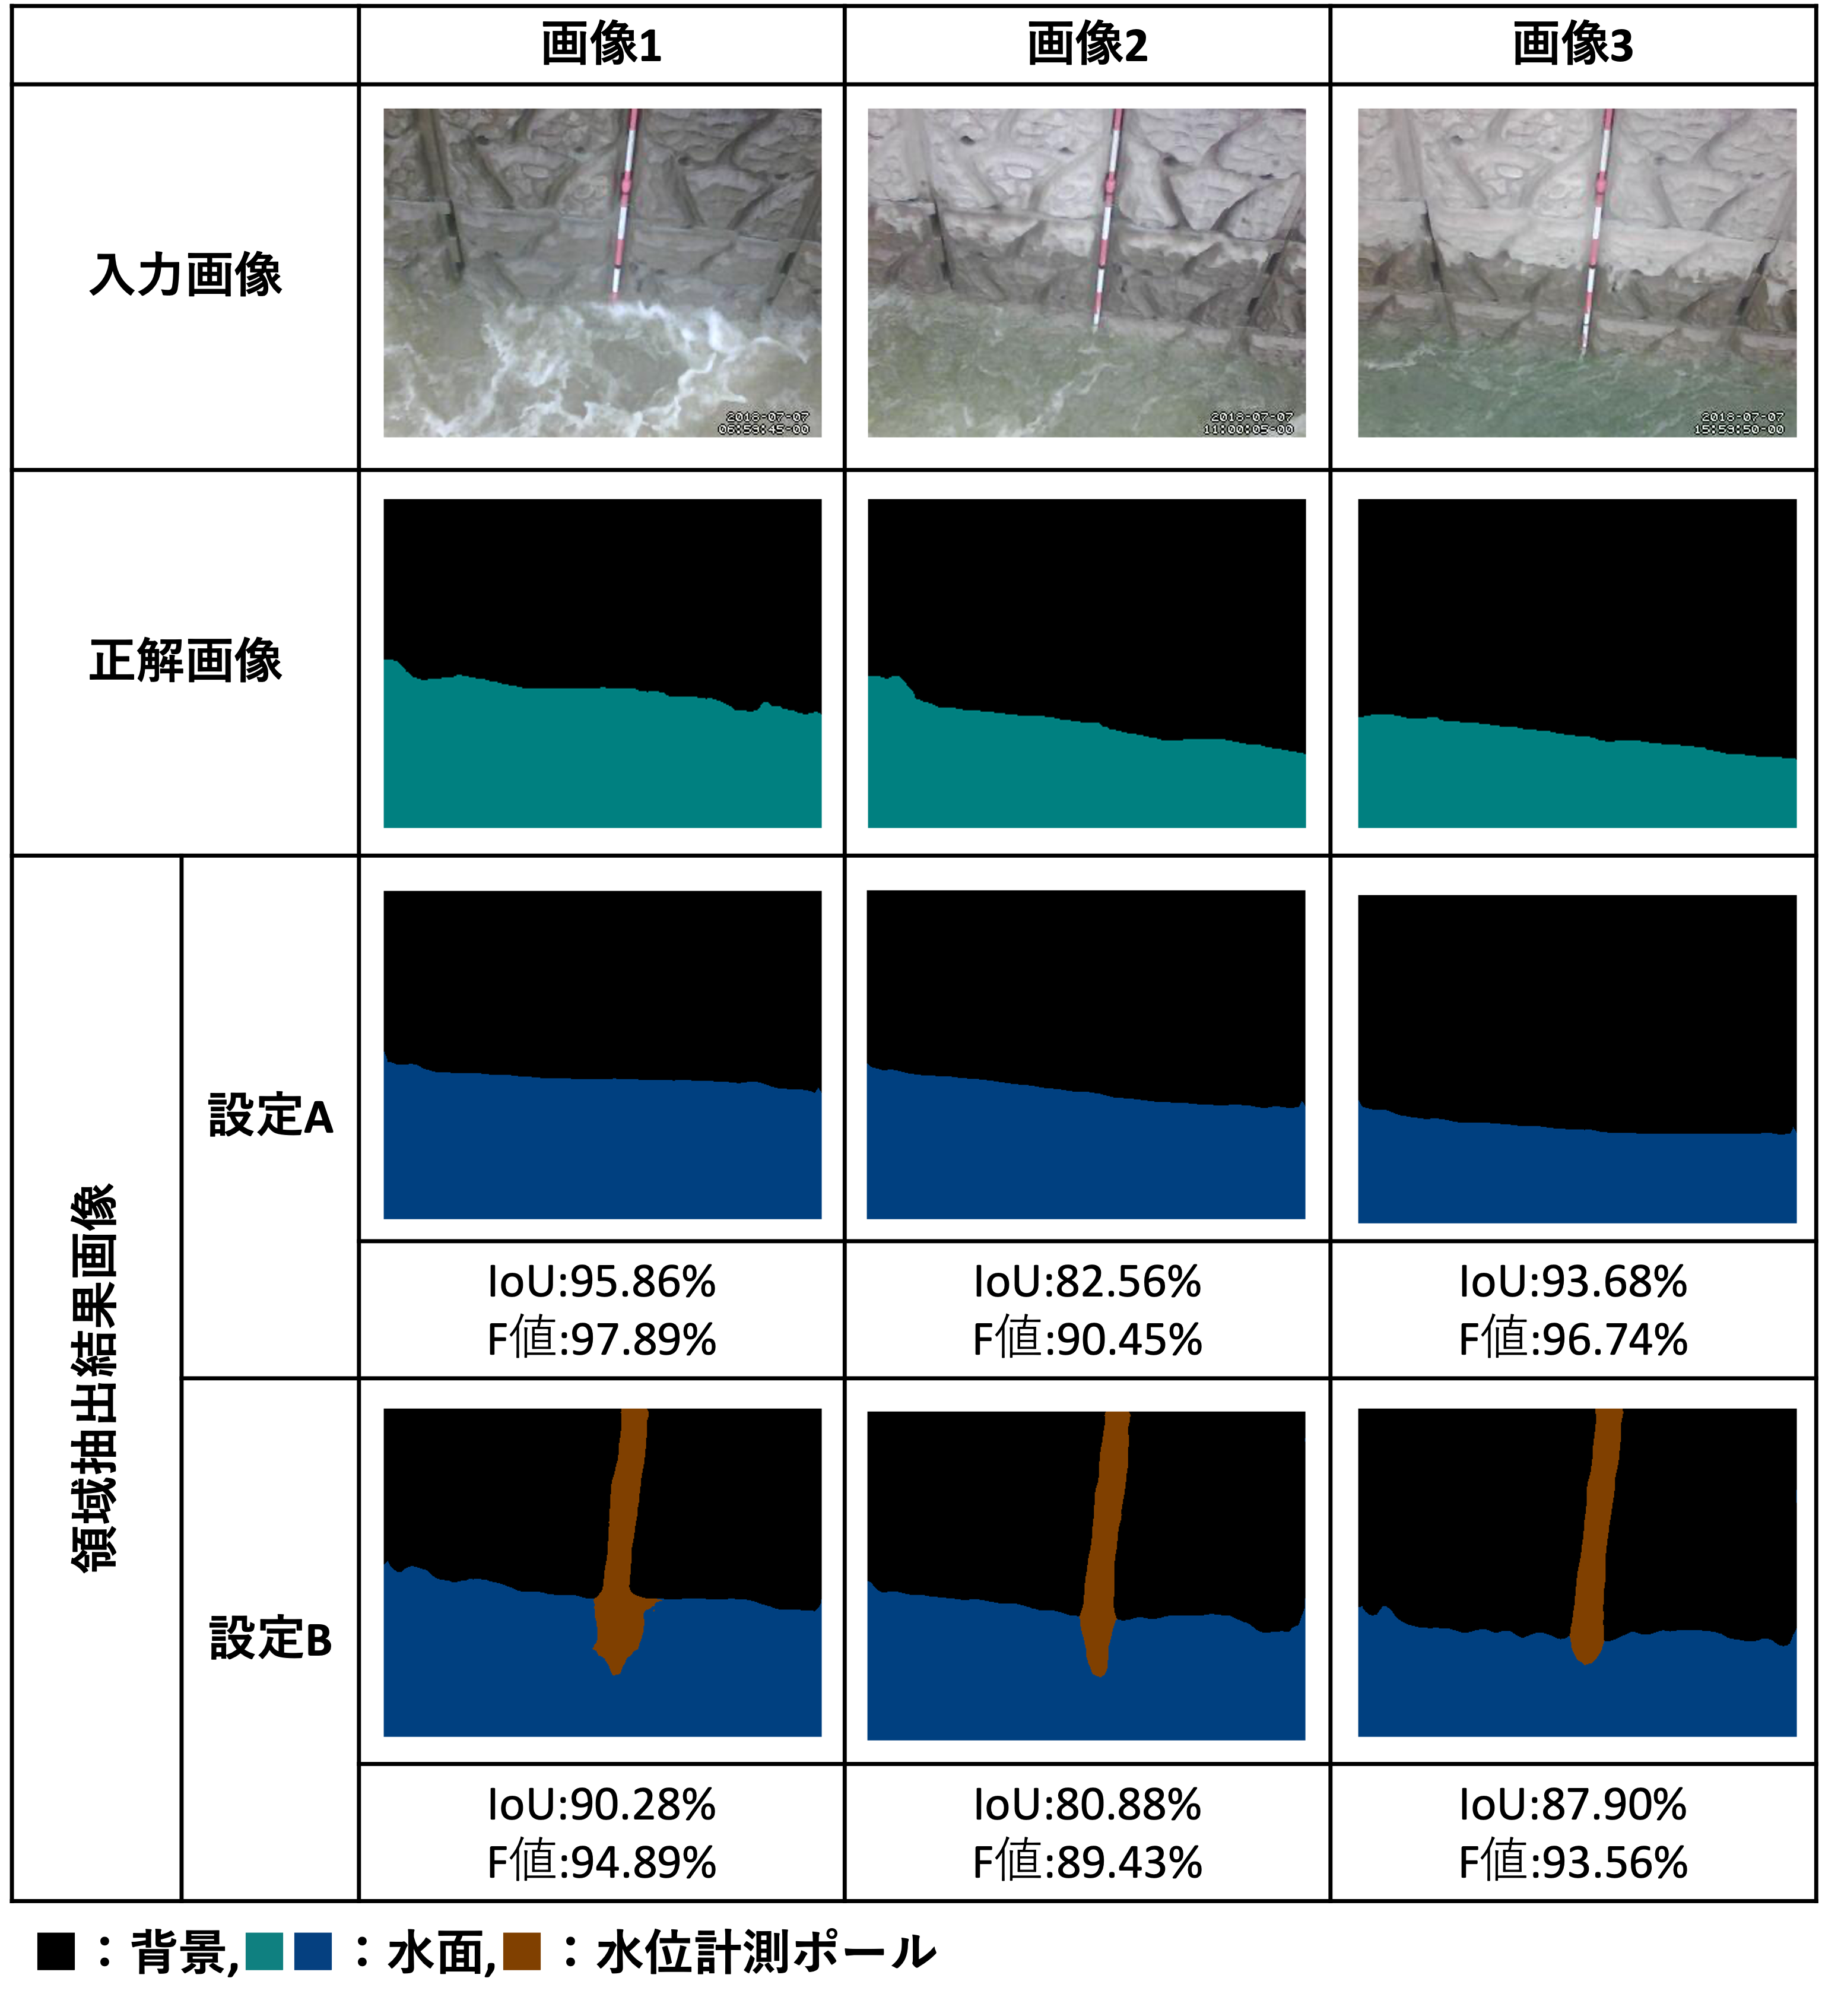
\includegraphics[width=0.9\linewidth]{image/image_pole.png}
  \end{center}
  \caption{領域抽出結果例}
  \label{AB_image}
\end{figure}
\clearpage

\subsection{先行研究\cite{watanabe}との比較}
\label{5.3}
SS手法の領域抽出精度を評価するため,時系列の河川の監視カメラ画像に
先行研究\cite{watanabe}の手法とSS手法を適応し,推定した水位と目視で計測した水位とのRMSEを比較した.
先行研究のラベル設定と統一するため,\ref{5.2}節より,
領域抽出精度が高かった設定Aでアノテーションを行った.
また,訓練データには7月6日の画像を,
テストデータには7月6日と7月7日の画像を使用した.

SS手法と先行研究の手法に対し,
水位を推定したとき,測定値とのRMSEは表\ref{senkou_ss}の通りとなった.
推定した水位を図\ref{ss_0706}から図\ref{senkou_0707}に示す.

\vspace{5mm}
\begin{table}[ht]
  \centering
  \caption{推定値と測定値のRMSE(cm)}  
  \begin{tabular}{lrr} \bhline{1.5pt}
     &7月6日&7月7日 \\ \hline 
   SS手法&8.05&  15.02\\ \hline  
   先行研究&26.00&  163.44\\ \hline  
  \end{tabular}
  \label{senkou_ss}
\end{table}


\begin{figure}[h] 
  \begin{center}
    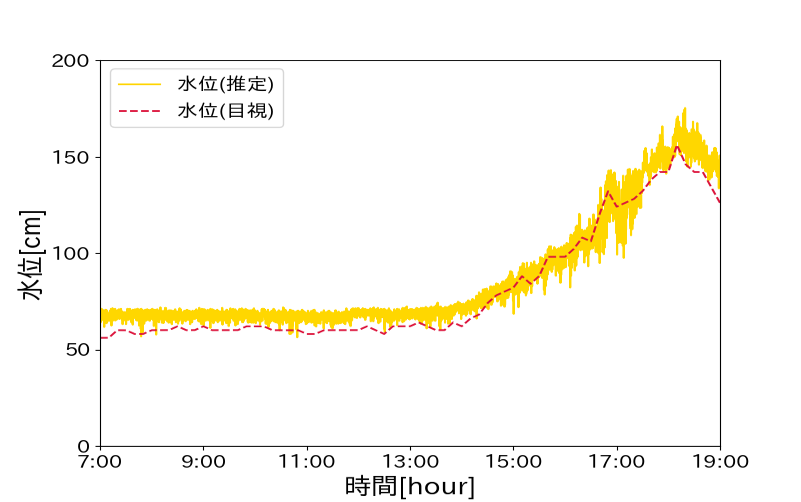
\includegraphics[width=\linewidth]{image/0706_ss.png}
  \end{center}
  \caption{SS手法の推定結果(テスト:7月6日)}
  \label{ss_0706}
\end{figure}


\begin{figure}[b] 
  \begin{center}
    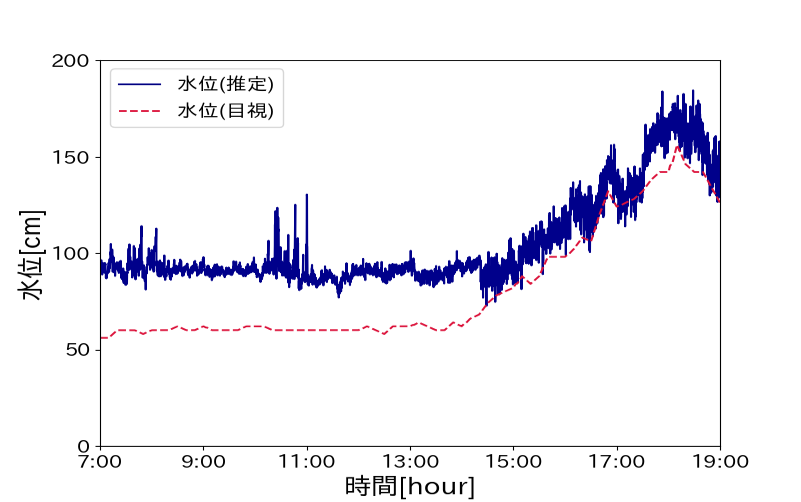
\includegraphics[width=\linewidth]{image/0706_senkou.png}
  \end{center}
  \caption{先行研究の手法の推定結果(テスト:7月6日)}
  \label{senkou_0706}
\end{figure}

\begin{figure}[h] 
  \begin{center}
    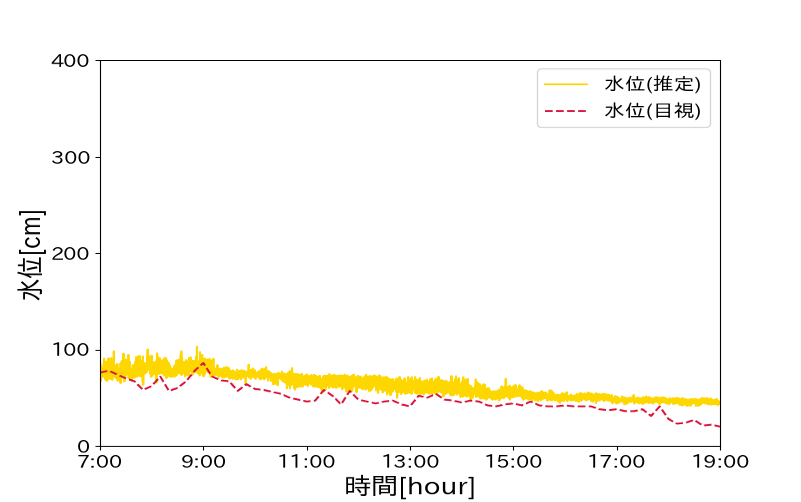
\includegraphics[width=\linewidth]{image/0707_ss.png}
  \end{center}
  \caption{SS手法の推定結果(テスト:7月7日)}
  \label{ss_0707}
\end{figure}

\begin{figure}[h] 
  \begin{center}
    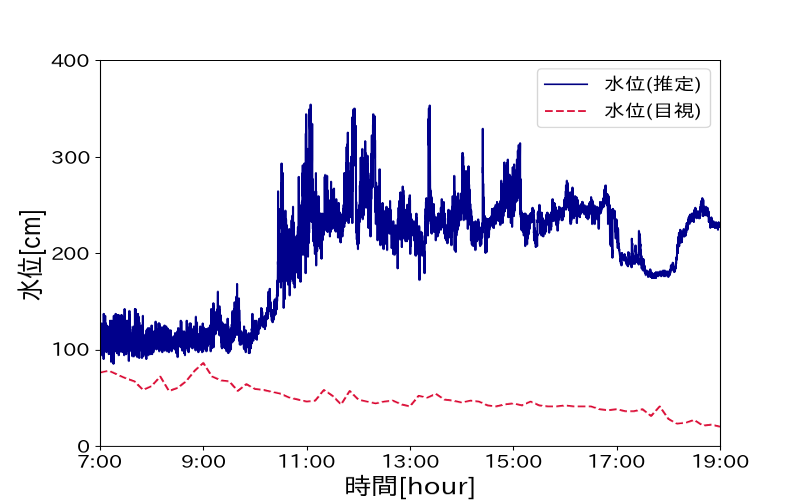
\includegraphics[width=\linewidth]{image/0707_senkou.png}
  \end{center}
  \caption{先行研究の手法の推定結果(テスト:7月7日)}
  \label{senkou_0707}
\end{figure}

%%%%%%%%%%%%%%%%%%%%%%%%%%%%%%%%%%%%%%%%%%%%%%
\clearpage
\section{考察}

\subsection{交差検証}
\label{6.1}

2018年,7月5,6,7日の3日分の画像データから
SS手法を用いて水位の推定を行った(3日分のデータの内,
2日分のデータを訓練データ,残った1日分のデータを
テストデータとして使用).
また,アノテーション設定は設定Aを使用した.

作成したモデルで推定した水位と測定値とのRMSEと領域抽出結果のIoU,F値は表\ref{kousa}の通りとなった. 
また,それぞれのテストデータ日の抽出結果例を図\ref{images_kousa}に示す.

表\ref{kousa}から,
提案手法を用いて作成したアノテーション画像を訓練に使用したモデルのIoUとF値は
すべてのテスト日で,85%以上を達成したことが確認できる.

7月5日の水位推定結果を図\ref{kousa_0705}に,時間別のIoUとF値を
図\ref{kousa_IoU_0705}に示す.
表\ref{kousa}より,7月5日は他の日と比較してRMSEが大きくなった.
また,7月5日の7:00から12:00の範囲で精度が低いことが
図\ref{kousa_0705}と図\ref{kousa_IoU_0705}から確認できる.
特に精度が低い抽出結果例を図\ref{images_kousa}の(b)に示す.
同じ,7月5日の画像である(a)の入力画像と(b)の入力画像から河川の状態を比べると,
(b)の入力画像は水面が低く,澄んでいることが確認できる.この現象によって,
水面と壁面の境界面が発見しにくくなり,領域抽出精度が下がったと考えられる.

7月6日の水位推定結果を図\ref{kousa_0706}に,時間別のIoUとF値を
図\ref{kousa_IoU_0706}に示す.
図\ref{kousa_IoU_0706}より,
15:00から17:00の間で領域抽出精度が低い瞬間があることが確認できる.
図\ref{images_kousa}の(d)にその瞬間の抽出結果を示す.
同日かつ,高精度で抽出が行えている(c)の入力画像と(d)の入力画像から河川の状態を比べると,
(d)の河川は水面が濁っていることが確認できる.
この現象によって,水面の輝度値が壁面と近くなり,領域抽出精度が下がったと考えられる.

7月7日の水位推定結果を図\ref{kousa_0707}に,時間別のIoUとF値を
図\ref{kousa_IoU_0707}に示す.
図\ref{kousa_IoU_0707}より,
7:00から9:00の間で領域抽出精度が低い瞬間があることが確認できる.
図\ref{images_kousa}の(f)にその瞬間の抽出結果を示す.
同日かつ,高精度で抽出が行えている
(e)の入力画像と(f)の入力画像から河川の状態を比べると,
(f)の河川は水面が波立っており,水面と壁面の境界が複雑になっていることが確認できる.
よって,水面の状態が大きく変化したことが,領域抽出精度が下がった要因だと考えられる.


\vspace{3mm}
\begin{table}[ht]
  \centering
  \caption{テストデータ日別RMSEと領域抽出精度}  
  \begin{tabular}{l|rrr} \bhline{1.5pt}
     &7月5日&7月6日&7月8日 \\ \hline 
   IoU(%)&88.33&91.05&90.36\\ \hline  
   F値(%)&93.76&95.26&94.87\\ \hline  
   RMSE(cm)&17.32& 7.73&8.32\\ \hline  
  \end{tabular}
  \label{kousa}
\end{table}
\clearpage

\begin{figure}[t] 
  \begin{center}
    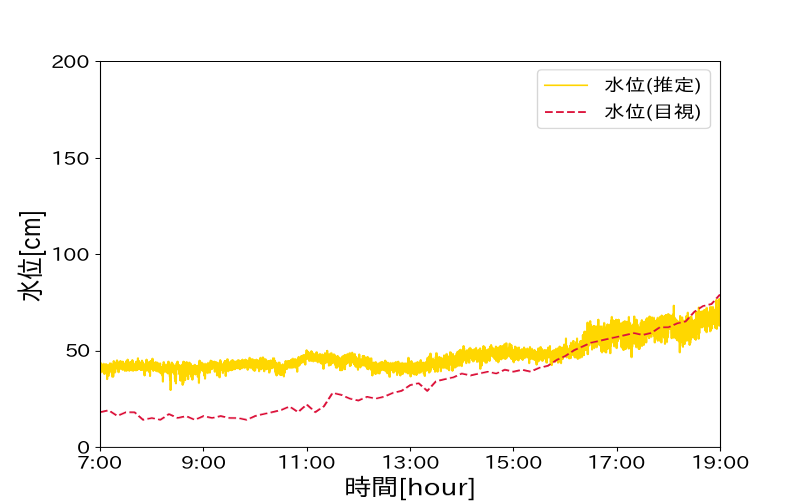
\includegraphics[width=\linewidth]{image/0705_kousa.png}
  \end{center}
  \caption{水位の推定結果(テスト:7月5日)}
  \label{kousa_0705}
\end{figure}

\begin{figure}[b] 
  \begin{center}
    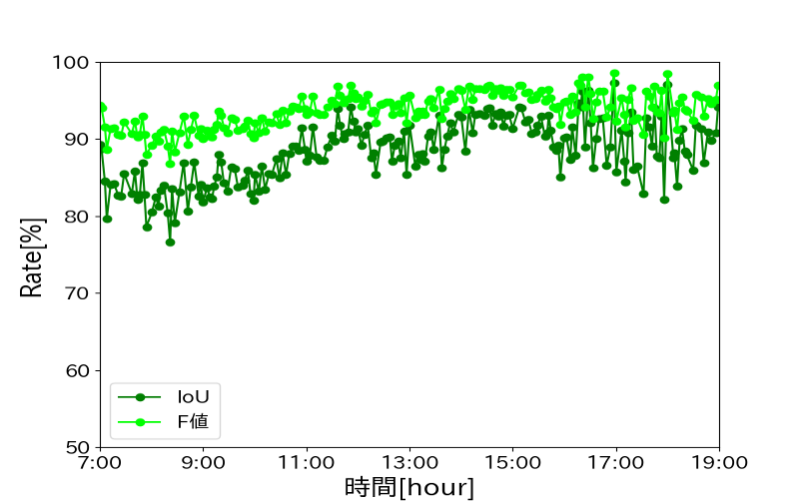
\includegraphics[width=\linewidth]{image/0705_f_IoU.png}
  \end{center}
  \caption{時間別IoU,F値(テスト:7月5日)}
  \label{kousa_IoU_0705}
\end{figure}


\begin{figure}[ht] 
  \begin{center}
    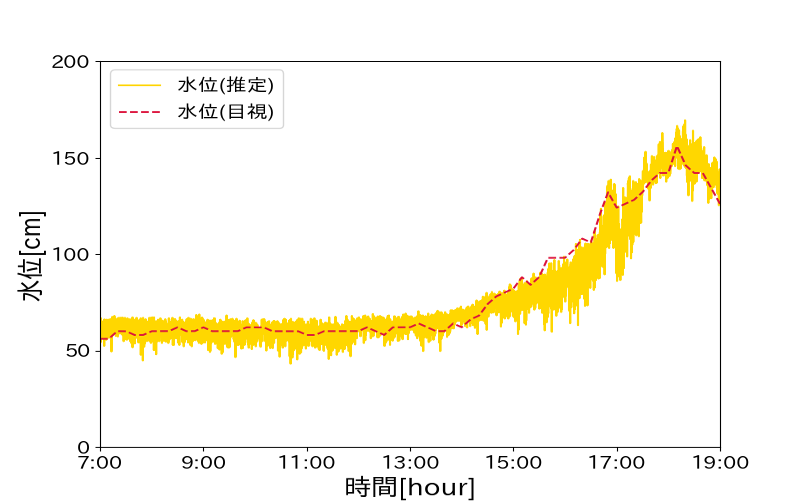
\includegraphics[width=\linewidth]{image/0706_kousa.png}
  \end{center}
  \caption{水位の推定結果(テスト:7月6日)}
  \label{kousa_0706}
\end{figure}

\begin{figure}[ht] 
  \begin{center}
    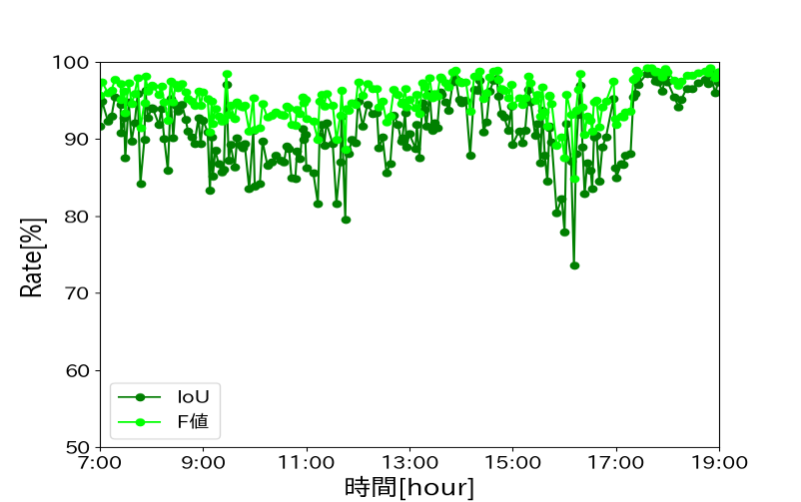
\includegraphics[width=\linewidth]{image/0706_f_IoU.png}
  \end{center}
  \caption{時間別IoU,F値(テスト:7月6日)}
  \label{kousa_IoU_0706}
\end{figure}


\begin{figure}[ht] 
  \begin{center}
    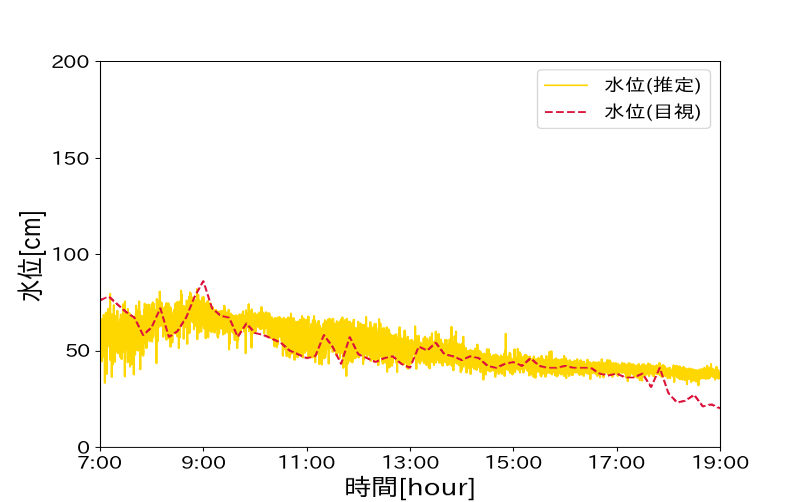
\includegraphics[width=\linewidth]{image/0707_kousa.png}
  \end{center}
  \caption{水位の推定結果(テスト:7月7日)}
  \label{kousa_0707}
\end{figure}

\begin{figure}[ht] 
  \begin{center}
    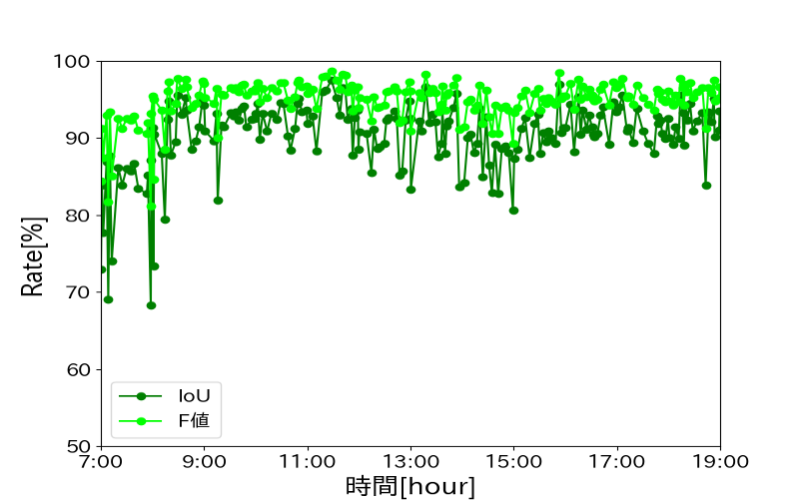
\includegraphics[width=\linewidth]{image/0707_f_IoU.png}
  \end{center}
  \caption{時間別IoU,F値(テスト:7月7日)}
  \label{kousa_IoU_0707}
\end{figure}

\begin{figure}[t] 
  \begin{center}
    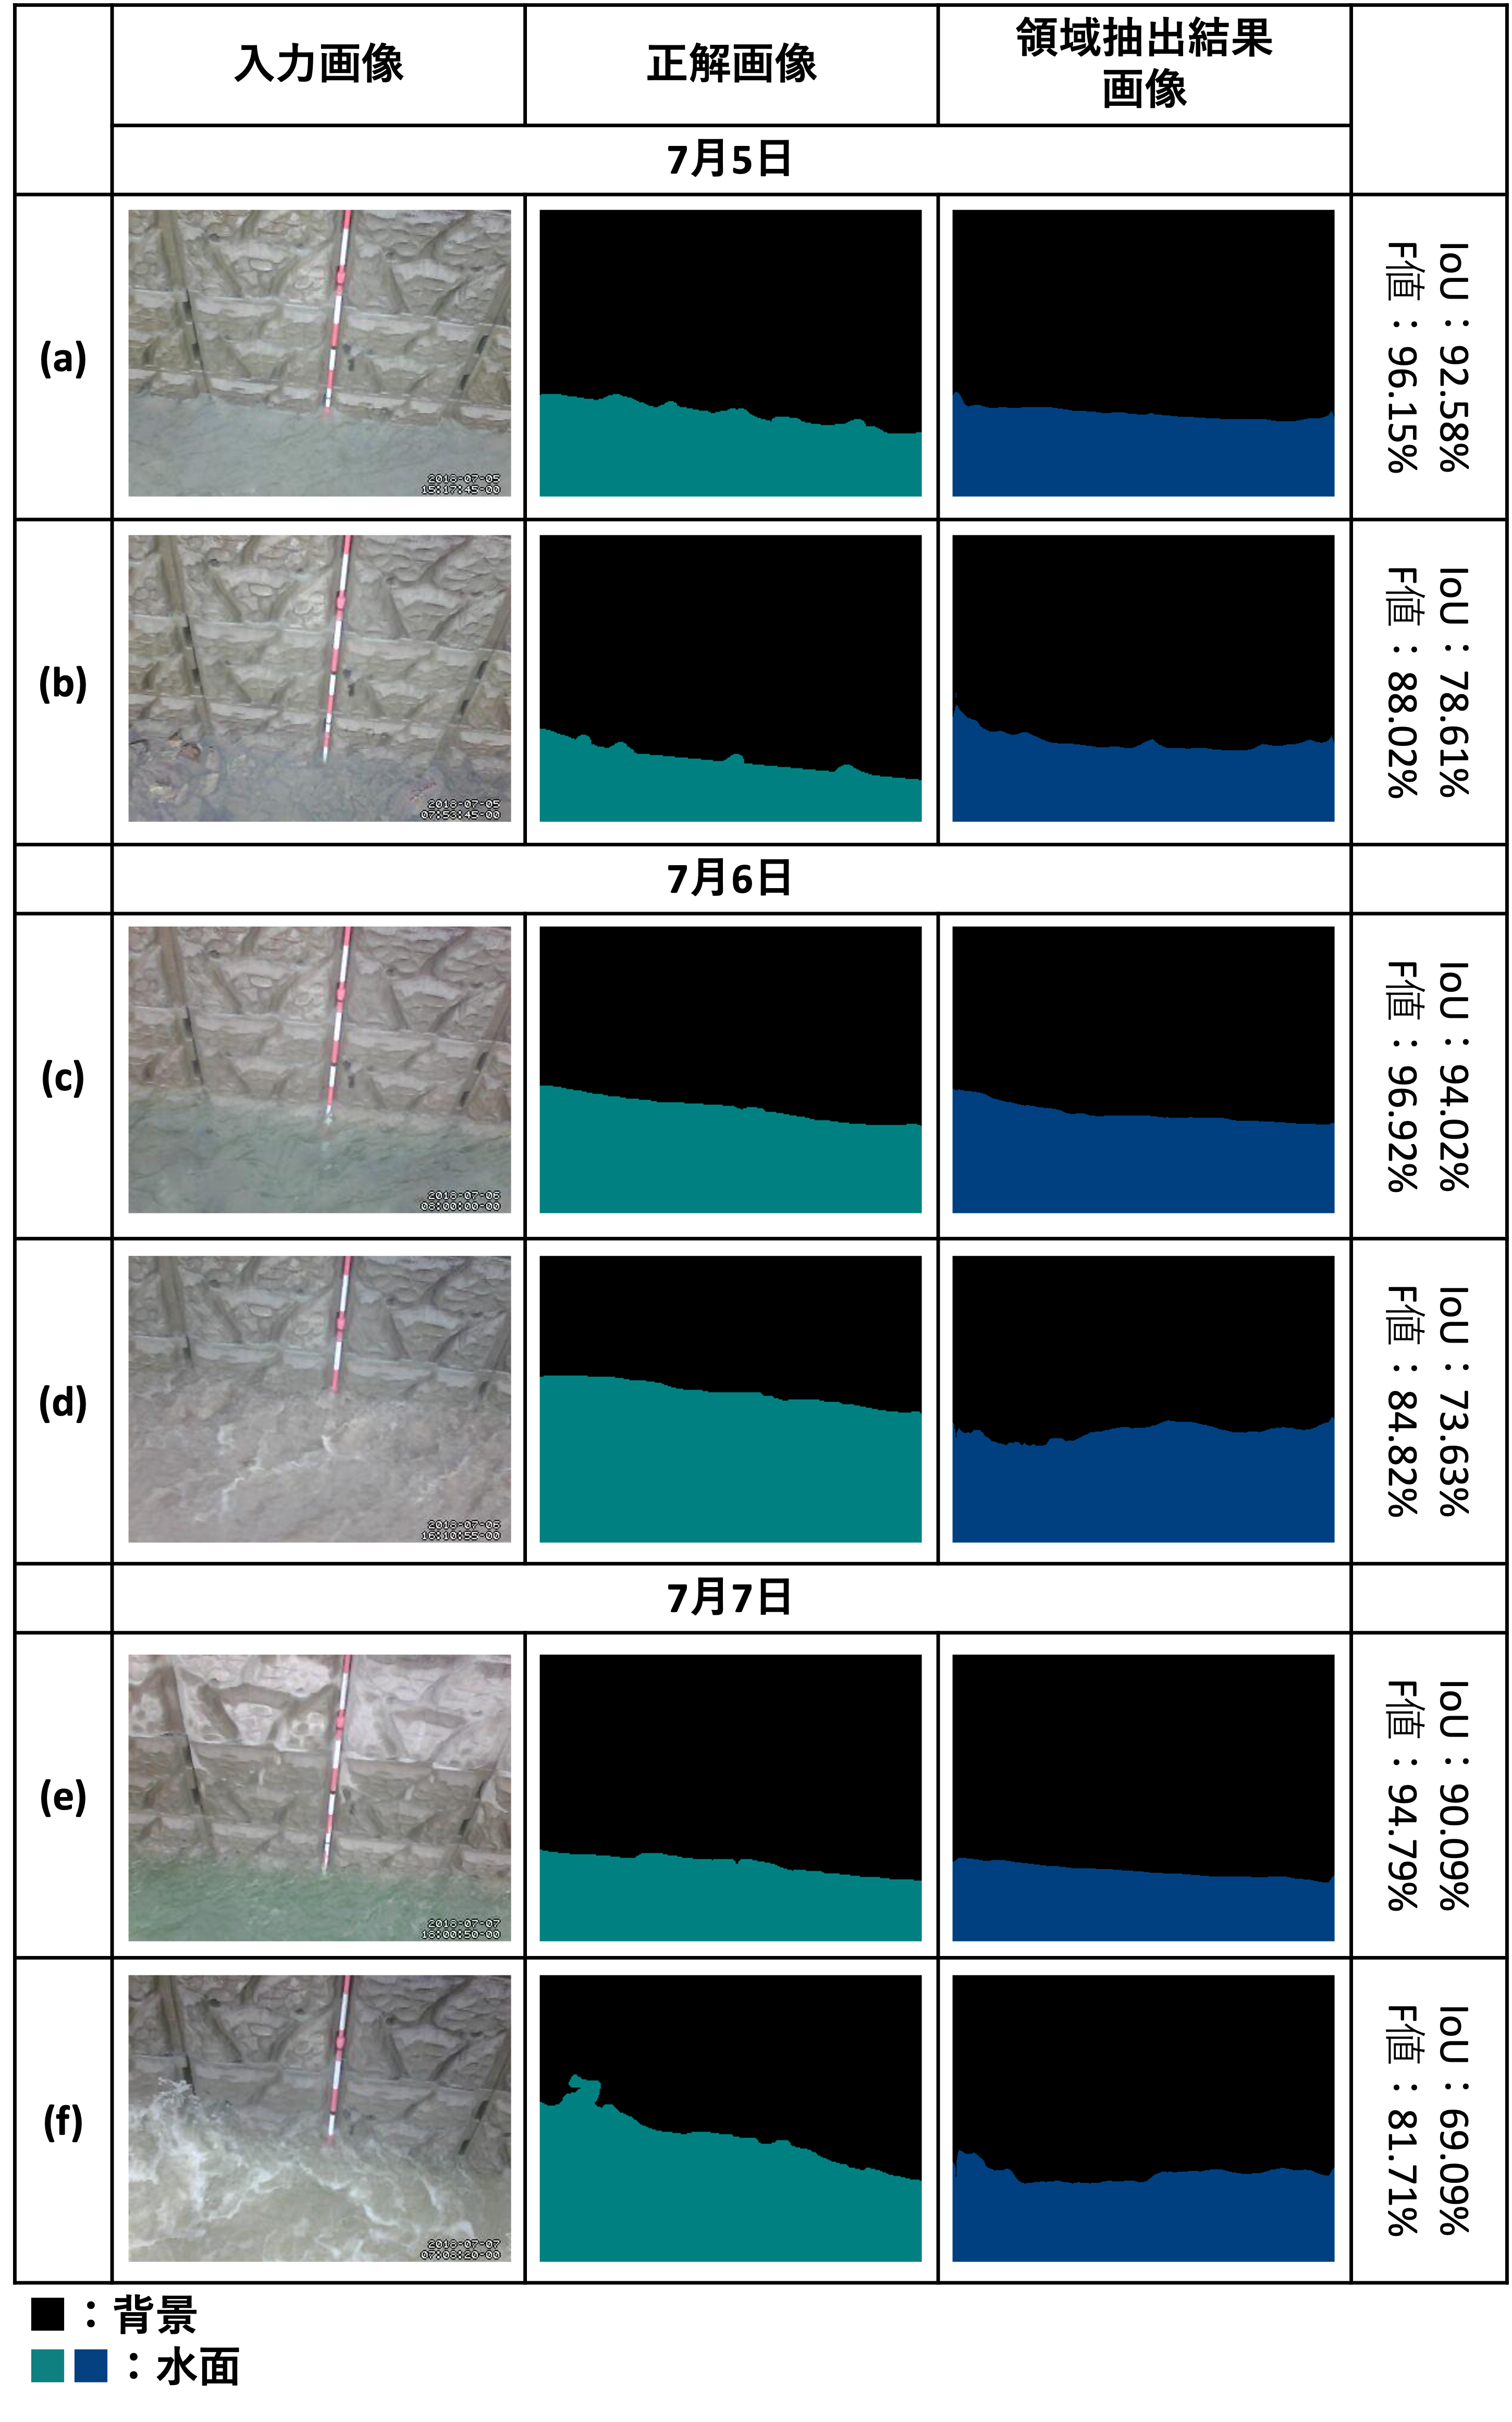
\includegraphics[width=120mm]{image/image_kousa.png}
  \end{center}
  \caption{領域抽出結果例}
  \label{images_kousa}
\end{figure}

\clearpage
\subsection{評価実験について}

5.1 節では,
セマンティックセグメンテーションモデルを
構築する最適な学習回数をモデルの領域抽出精度
から調査した.図\ref{kousa}より,200回からIoUとF値
は収束していることが確認できた.したがって,モデルの学習回数は最低でも
200回以上必要であるといえる.

5.2節では,2種類のアノテーション設定で構築したモデルの領域抽出精度を
IoUとF値で比較した.
表\ref{pole},図\ref{AB_IoU},図\ref{AB_bf}より,
設定Aの方がIoUとF値が良い結果になることが確認できた.
図\ref{AB_image}の領域抽出結果例から,
水位計測ポールに水位計測ポールラベルを与えた場合,
水面領域に覆いかぶさる形で水位計測ポールの推定を行っていることが確認できる.
このような推定により,水面の領域抽出精度が低くなったと考えられる.

5.3節では,SS手法を用いて推定した水位と目視で計測した水位とのRMSE
を先行研究の手法の結果と比較した.表\ref{senkou_ss}より,SS手法を用いた場合 
の方がRMSEは小さくなった.

\subsection{先行研究\cite{seman}との比較}
先行研究\cite{seman}は本研究と同じく,
セマンティックセグメンテーションを用いて
河川の監視カメラ画像から水面領域を抽出し,水位の推定を行っている.
しかし,本研究と比較してアノテーション方法,水位の推定方法,評価方法に相違点が見られた.

先行研究\cite{seman}は
MATLABソフトウェアのImage Labelerツールを用いて半自動でアノテーション画像を
作成した.
元画像にラベル付けした画像を図\ref{seman_ano}に示す.
図\ref{seman_ano}から,
先行研究cite{seman}も本研究の設定Aと共通して,水面と背景の2種類のラベルを使用していることが確認できる.
しかし,学習除外領域の設定を行わず,
水面と背景の境界面付近を細かくラベル付けを行っている点は本研究と異なる.

先行研究\cite{seman}は本研究と異なる水位推定方法を用いている.
先行研究は図\ref{level}に示す閾値マーカーに焦点を当て,水位の推定を行った.
閾値マーカーは,Normal(緑),Alert(黄),Warning(橙),Danger(赤)の4種類である.
領域抽出した結果,水面と背景の境界面が二つの閾値マーカーの間に
存在すると推定された場合は二つの閾値の平均値を水位とし,
また,境界面が閾値マーカー上にあると推定された場合は閾値の値を水位とした.

本研究は,推定した水位と測定した水位とのRMSEを先行研究\cite{watanabe}と比較することで,
セマンティックセグメンテーションを用いた水位推定の評価を行った.
一方,先行研究\cite{seman}は5日間の水位推定を行い,推定値とセンサーで取得した水位との相関を
利用して評価を行った.


\begin{figure}[h] 
  \begin{center}
    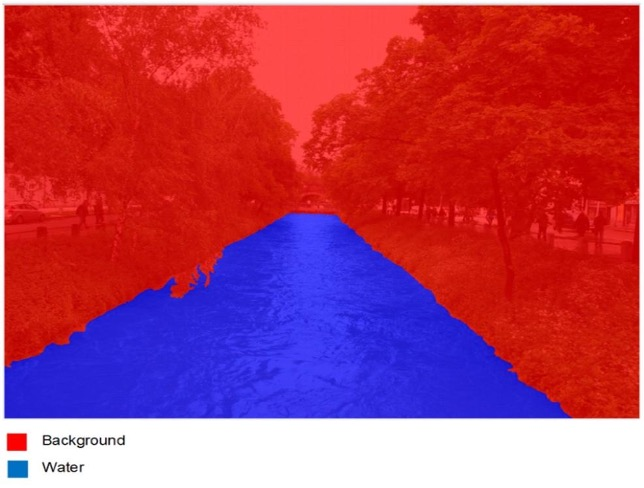
\includegraphics[width=0.8\linewidth]{image/n_iamge.jpg}
  \end{center}
  \caption{ラベル付き画像}
  \label{seman_ano}
\end{figure}
\begin{figure}[ht]
  \centering
  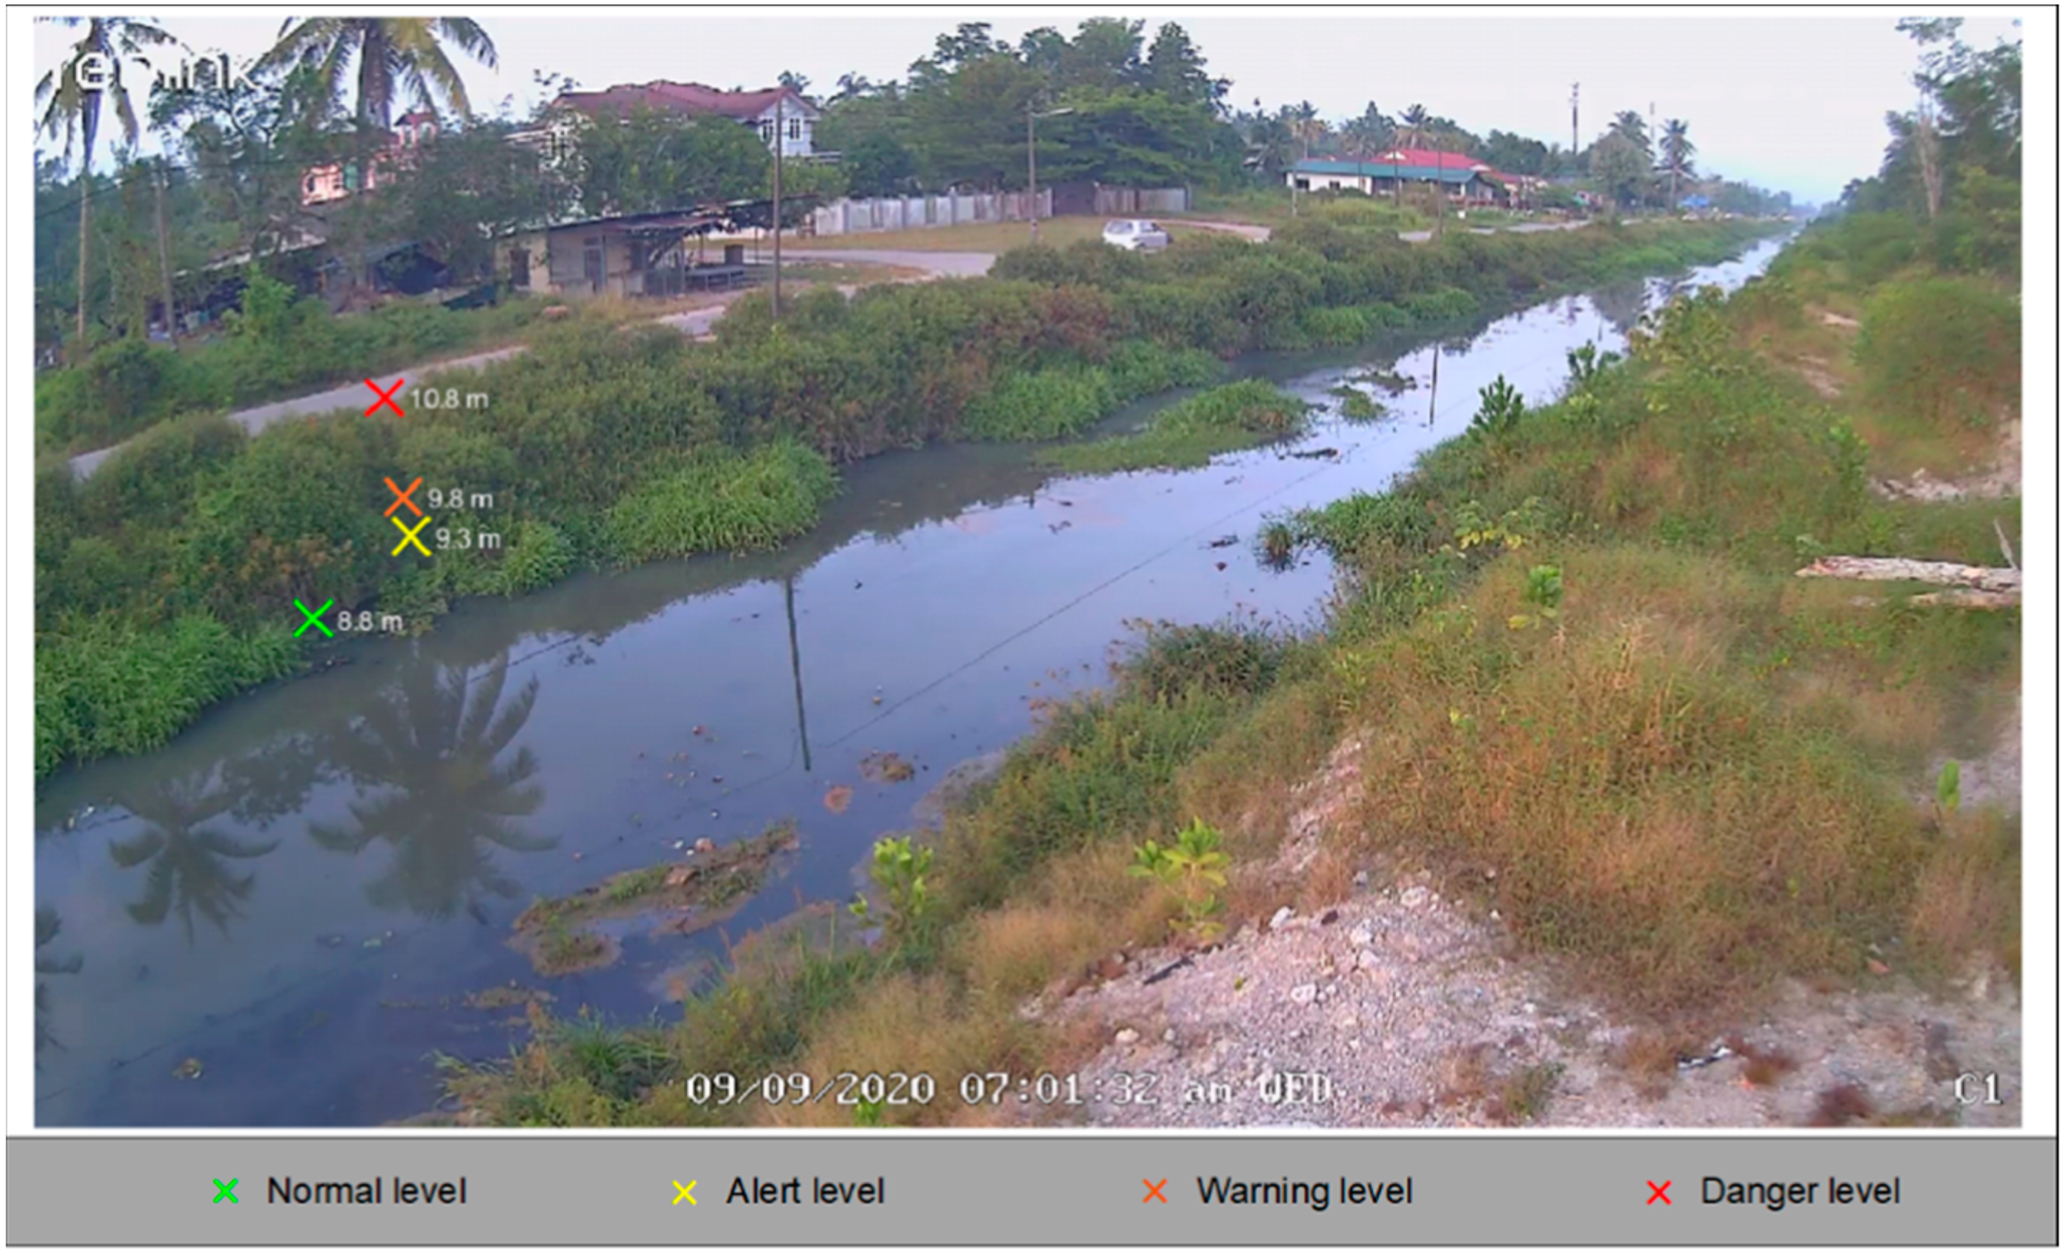
\includegraphics[width=0.8\linewidth]{image/n_level.png}
  \caption{閾値マーカー}
  \label{level}
\end{figure}
\clearpage
%%%%%%%%%%%%%%%%%%%%%%%%%%%%%%%%%%%%%%%%%%%%%%
\section{まとめ}
\label{7}
本研究では,深層学習を用いたセマンティックセグメン
テーションによって河川の監視カメラ画像から水位を推定することを目的とし,
訓練データとして必要なアノテーション画像を半自動的に作成する方法を提案した.
交差検証を行った結果,提案手法を用いて作成したモデルは全て
のテスト日でIoUとF値が85%以上となった.
しかし,水面の状態によって精度が低くなるといった問題が見受けられた.
また,水位の推定方法としてSS手法を用いた手法を検討した.
SS手法と先行研究の手法を適用して水位を推定し,
目視で測定した水位との誤差を利用して評価を行った.
その結果,SS手法のRMSEが15.02cm,先行手法が163.44cmとなり,
SS手法を用いた場合の誤差の方が小さくなった.
今後の課題としては,他の河川に対する適用実験やアノテーション画像の自動生成などが
挙げられる.


%本文ここまで
\clearpage

%参考文献
\addcontentsline{toc}{section}{\refname}
\begin{thebibliography}{99}
  \bibitem{mlit}
  国土交通省:
  令和4年の土砂災害発生件数は795件,
  砂防NEWS Press Release,(2023年3月).

  \bibitem{zentyou}
  国土交通省水管理・国土保全局砂防部 : 
  「土砂災害警戒避難に関わる前兆現象情報の活用のあり方について」, 
  \url{http://www.mlit.go.jp/common/001021004.pdf}, (2006年3月). 



  \bibitem{watanabe}
  渡邊 康平:
  土砂災害の前兆現象検知を目的とした画面分割と深層学習を用いた水位変動の推定,
  広島市立大学大学院情報科学研究科システム工学専攻修士論文,
  (2023年1月). 

  \bibitem{seman}
  Nur Atirah Muhadi ,Ana Mijic , Ahmad Fikri Abdullah ,
  Siti Khairunniza Bejo , Muhammad Razif Mahadi: 
  Deep Learning Semantic Segmentation for Water Level Estimation Using Surveillance Camera,
  Applied Sciences,vol.11,issue.20,(2021).

  \bibitem{deeplabv3+}
  Chen, L. C., Zhu, Y., Papandreou, G., Schroff, F.,Adam, H. :
  Encoder-decoder with atrous separable convolution for semantic image segmentation. 
  In Proceedings of the European conference on computer vision (ECCV) (pp. 801-818).(2018).

  \bibitem{segnet}
  Badrinarayanan, V., Kendall, A.,Cipolla, R.:
  Segnet: A deep convolutional encoder-decoder architecture for image segmentation. 
  IEEE transactions on pattern analysis and machine intelligence, 39(12), 2481-2495.(2017).

  \bibitem{IoU}
  青島亘佐, 山本拓海, 中野聡,中村秀明:
  深層学習によるセグメンテーション手法を用いたコンクリート表面の変状領域の検出.
  AI・データサイエンス論文集, 1(J1), 481-490.(2020年).
  
  \bibitem{bf}
  山根達郎,全邦釘: 
  Deep learning による Semantic Segmentation を用いたコンクリート表面ひび割れの検出. 
  構造工学論文集 A, 65, 130-138.(2019年).

\end{thebibliography}

\newpage
\addcontentsline{toc}{section}{謝辞}
\section*{謝辞}
本研究に関して多大なるご指導を頂きました広島市立大学情報科学研究部システム工学科の島和之准教授に心より御礼申し上げます.
平素より島准教授には,研究の進め方について丁寧にご指導とご鞭撻を賜りました.重ねて感謝いたします.
また,本実験で使用する河川の画像をご提供くださいました
同学情報工学専攻センシング講座西正博教授に厚く感謝申し上げます.


\end{document}
